\documentclass[10pt]{article}
\usepackage[margin=1in]{geometry}
 \usepackage{auto-pst-pdf}
\usepackage{graphicx}
\usepackage{footnote}
%\usepackage{arydshln}
\usepackage{ifpdf}
\ifpdf
  \usepackage{epstopdf}
\fi
\usepackage{multirow}
\usepackage{epsfig}
\usepackage{float}
\usepackage{url}
\usepackage{color}
\usepackage{comment}
\usepackage{subfigure}

%\newcommand\solidrule[1][1cm]{\rule[0.5ex]{#1}{.4pt}}
%\newcommand\dashedrule{\mbox{%
%  \solidrule[2mm]\hspace{2mm}\solidrule[2mm]\hspace{2mm}\solidrule[2mm]}}
  
%\usepackage{hyperref}

\begin{document}
\title{Characterizing Execution Times on Realistic Programs}

\author{
Database \& Big Data Systems Laboratory,\\
School of Computer Science and Engineering, \\
Kyungpook National University,\\
Young-Kyoon Suh\\
}
\maketitle

\section{Description}
This document characterizes execution times 
measured on several real-world programs with different input sizes. 
To achieve this characterization, we discuss 
various histograms of execution times, measured in program time (PT), of the programs throughout this document. 
In this work we wish to achieve several goals as follows. 
The first goal is to unravel any structure behind the histograms and present insights into how such structure is formed. 
Another goal is to build a statistical distribution (or model) fitting in the histograms. 
From that distribution, we may reach predicting a concrete execution time considering system noise via 
the model on an arbitrary algorithm with a given input on a real execution environment. 
As a note, the execution times were measured along with the EMPv5~\cite{EMP} protocol. 
%In the protocol, we use taskstats C struct to get measures of a captured process. 
%The taskstat's data is delivered via a netlink socket from the kernel space. 
%The receive buffer for the socket is not robust for many observed processes~\cite{Metrology}. 
%Fortunately, there is an average of 95 processes per iteration of a run, 
%which turns out to be fine with the struct. 
%For a much more number of processes, 
%the use of  {\tt /proc/}[pid]{\tt{/stat}} is preferred, 
%as (i) there are equivalent measures available in the {\tt /proc} filesystem, 
%and (ii) there's little constraint on the use as opposed to taskstats. 

The following section shows histograms for runs on 
different real-world programs with varying input sizes.

\section{Histograms of the Execution Times on Real-World Programs~\label{sec:real-world}} 

In this section we run three kinds of programs: {\it nested for-loop}, {\it insertion sort} and {\it matrix multiplication}. For the runs of the latter two programs, we varied their input sizes by 2{\small $\times$} while trying some intermediate sizes increased by $\sqrt{2}$ and measured execution times of the programs over each input size. We then exhibit different kinds of histograms in the subsequent sections.

\subsection{Inter-machine Repeatability Check~\label{sec:diff_machine}} 

In this section we check if the use of different machines affects the distribution of execution (process) times on the same program. 
In other words, we examine {\em inter-machine repeatability}. For this examination, we use the nested for loop program 
with different task lengths: 16 seconds, 13 seconds, and 17.2 seconds, termed {\em INC16}, {\em INC13}, and {\em INC17.2}, respectively. 

Figures~\ref{fig:dm_1}, ~\ref{fig:dm_2}, and ~\ref{fig:dm_3} display the process time (PT) histograms on INC16, INC13, and INC17.2 run on our machines (from {\tt sodb8} to {\tt sodb12}), respectively.

\begin{figure}[h]
	\centering
	\subfigure[PT frequency on INC16]{
		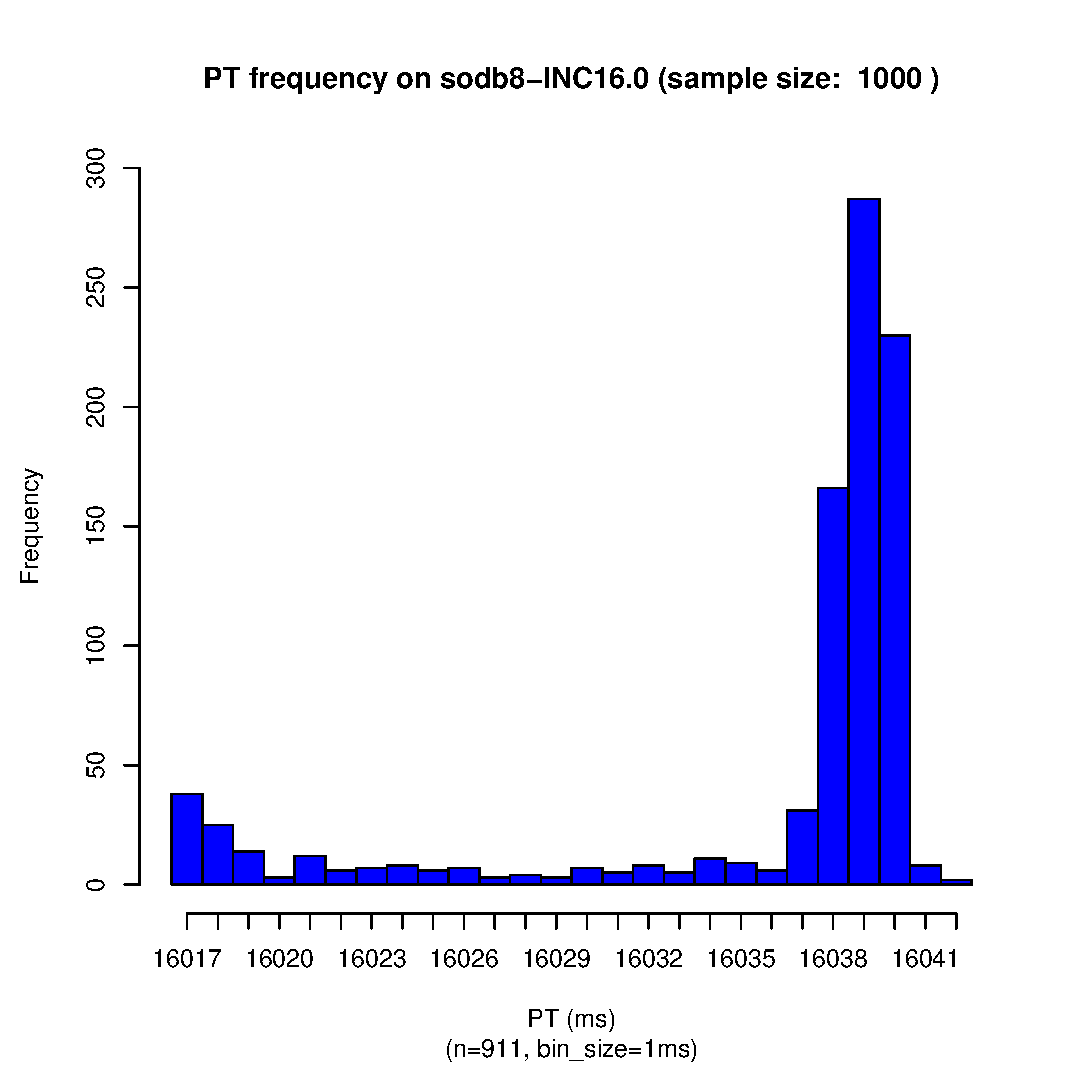
\includegraphics[scale=0.43]{sodb8_INC16_0_dist.eps}
		\label{fig:s8_inc16_dist}
	}	
	\subfigure[PT frequency on INC16]{
		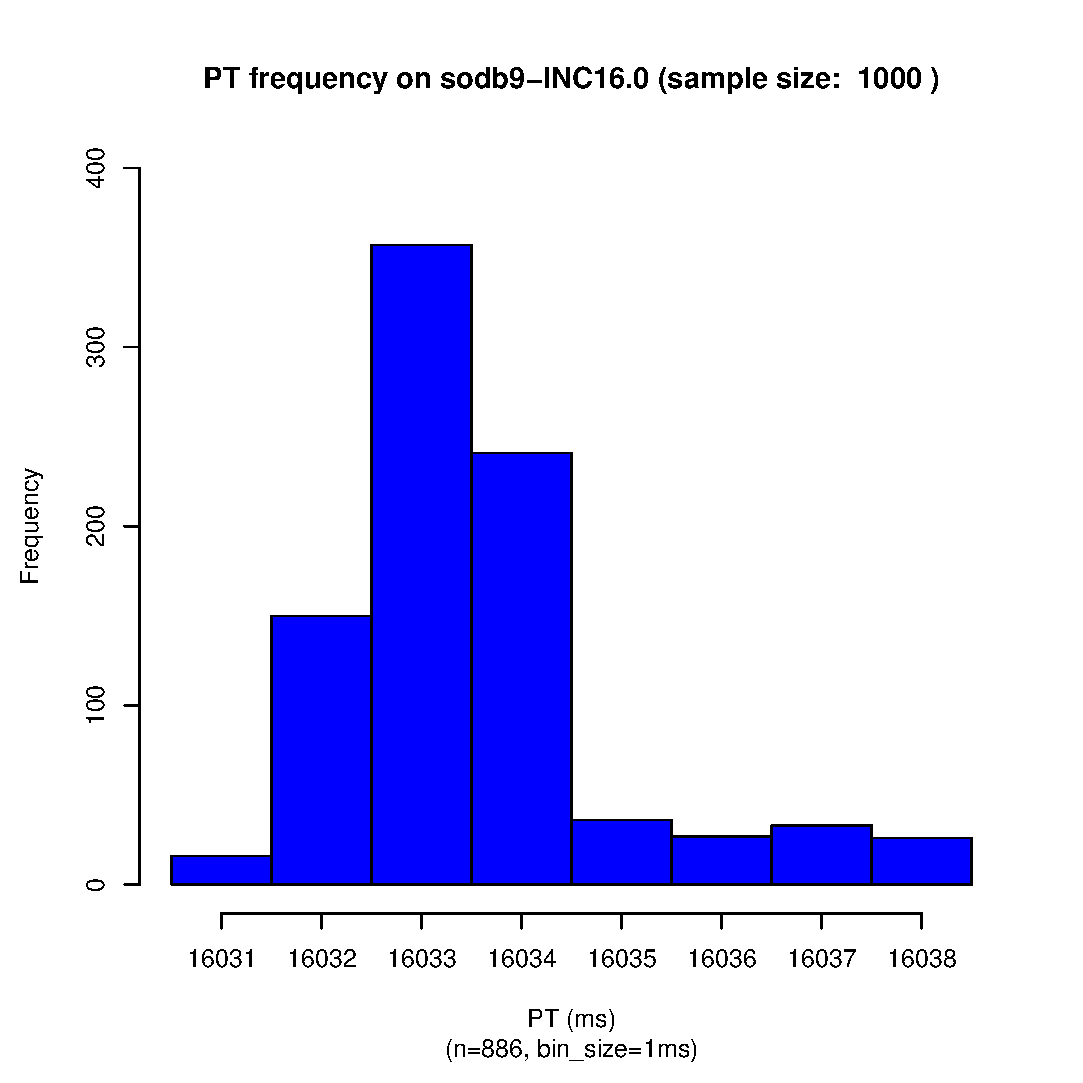
\includegraphics[scale=0.43]{sodb9_INC16_0_dist.eps}
		\label{fig:s9_inc16_dist}
	}
	\subfigure[PT frequency on INC16]{
		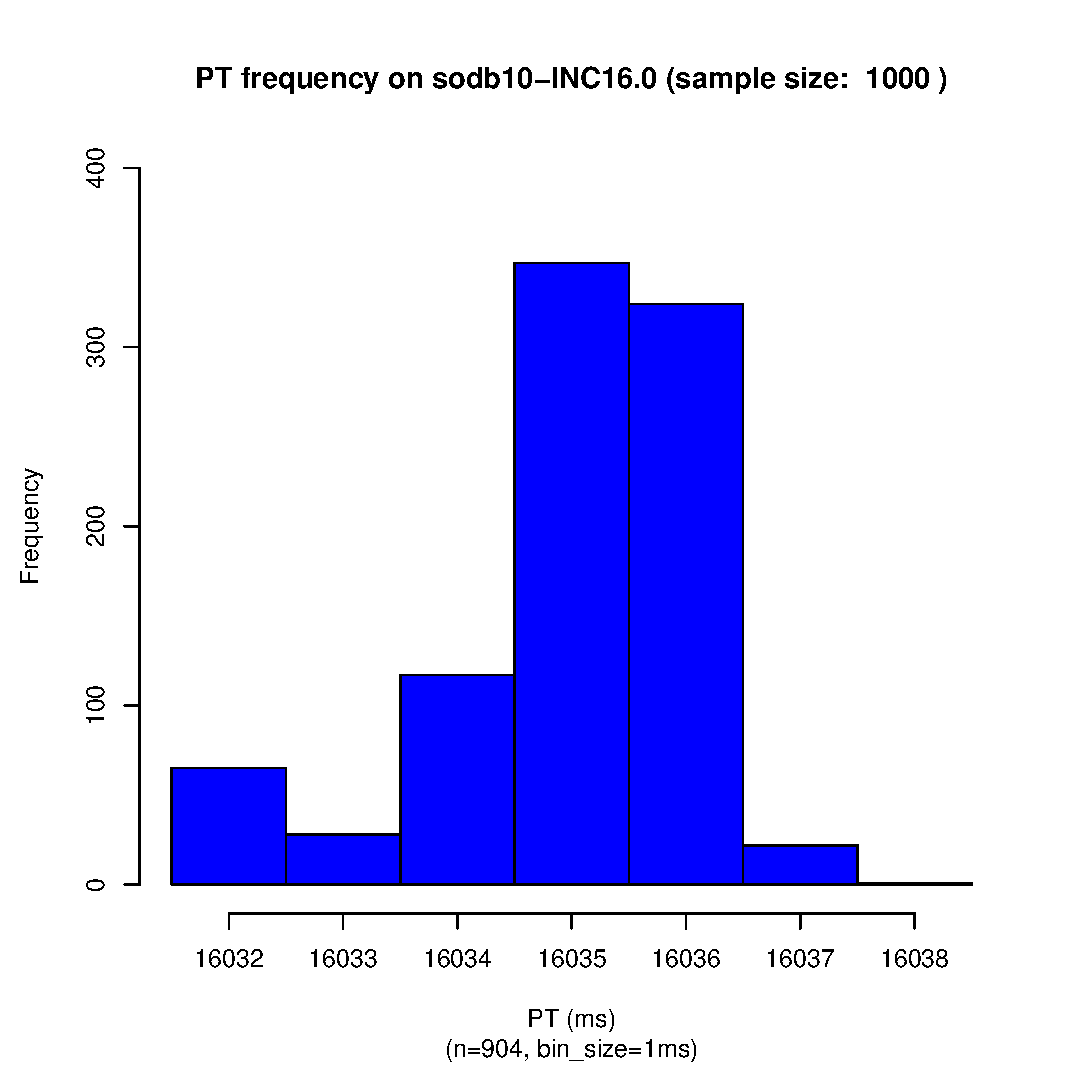
\includegraphics[scale=0.43]{sodb10_INC16_0_dist.eps}
		\label{fig:s10_inc16_dist}
	}	
	\subfigure[PT frequency on INC16]{
		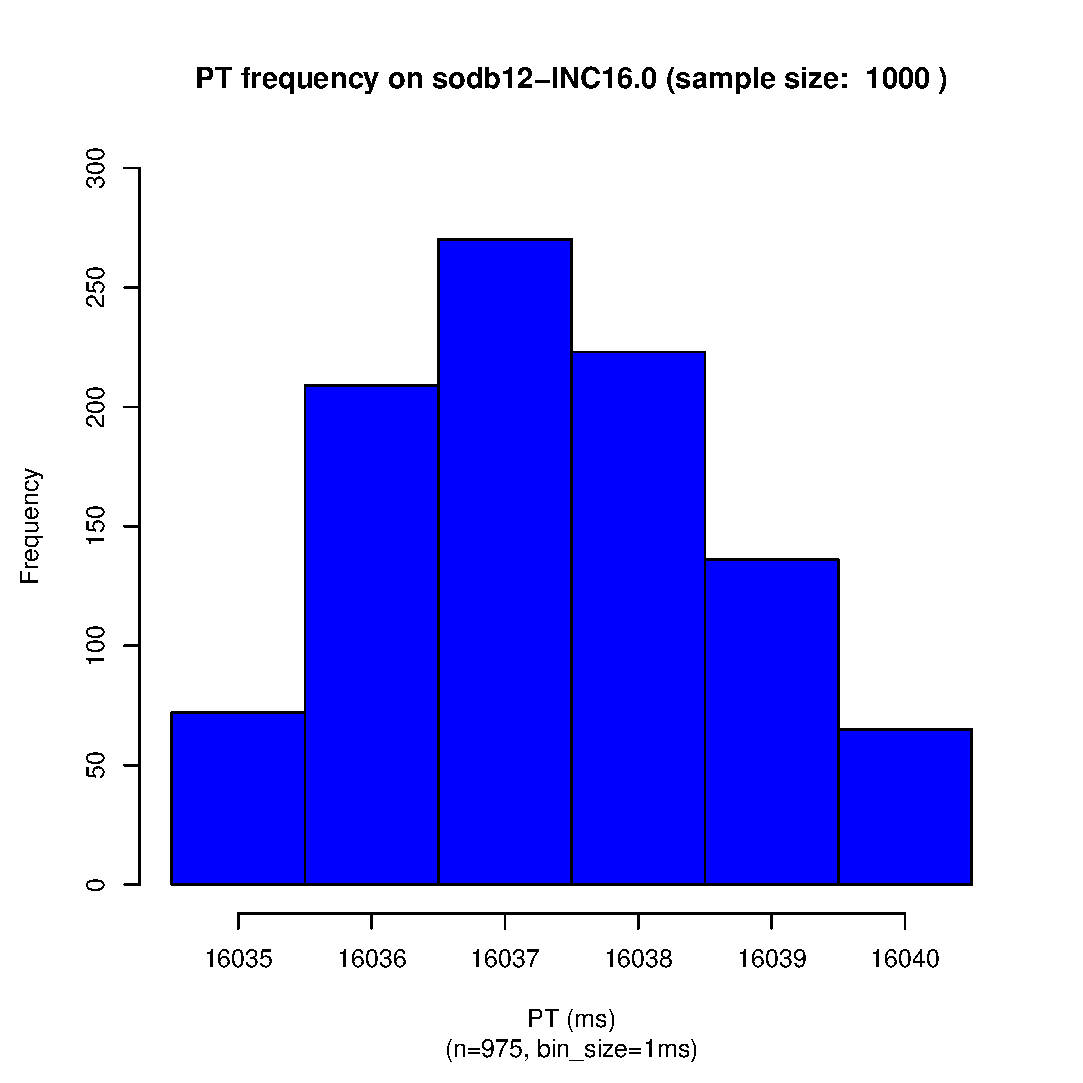
\includegraphics[scale=0.43]{sodb12_INC16_0_dist.eps}
		\label{fig:s12_inc16_dist}
	}
	\caption{PT Histograms on INC16~\label{fig:dm_1}}
\end{figure}

\newpage
\clearpage

\begin{figure}[h]
	\centering
	\subfigure[PT frequency on INC13]{
		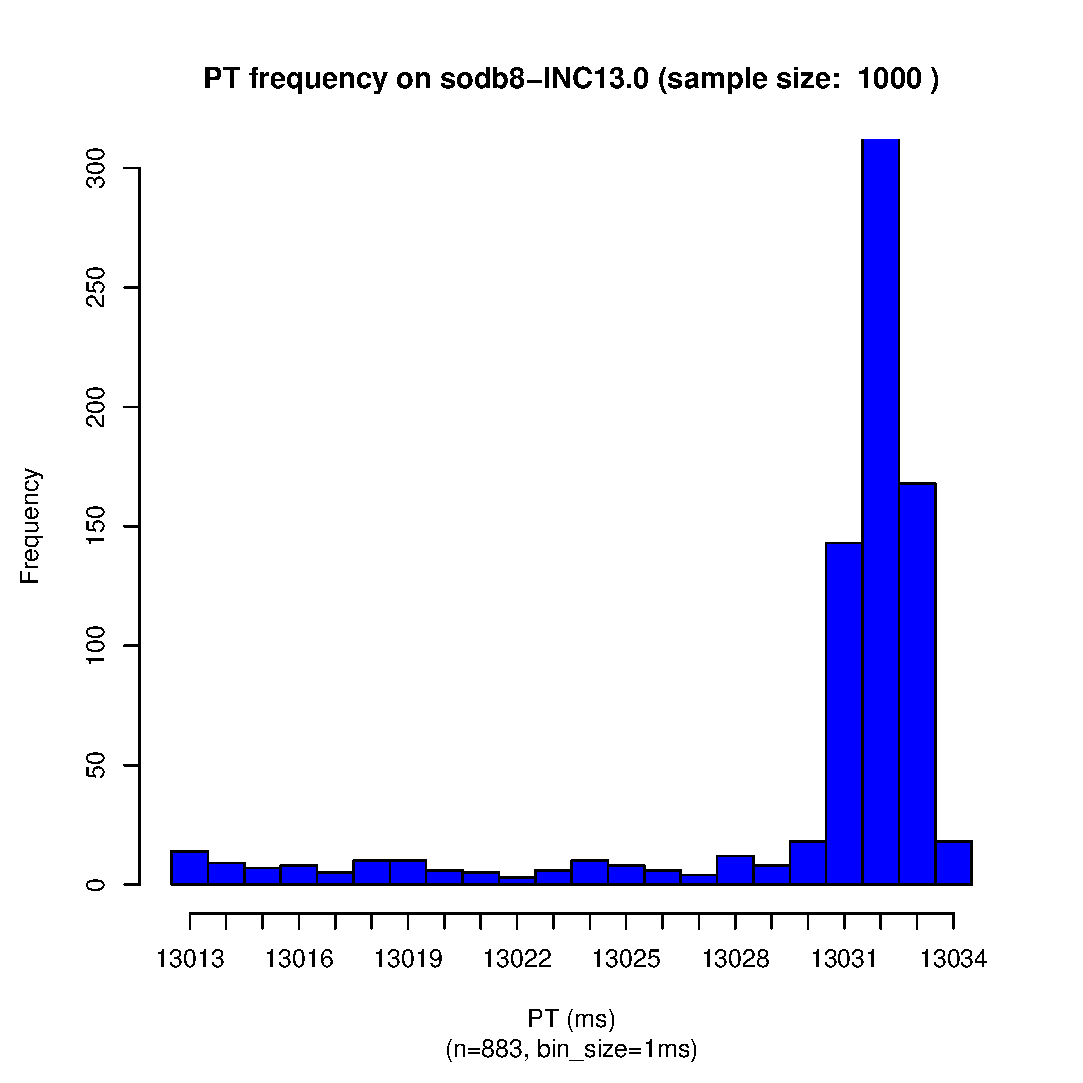
\includegraphics[scale=0.43]{sodb8_INC13_0_dist.eps}
		\label{fig:s8_inc13_dist}
	}	
	\subfigure[PT frequency on INC13]{
		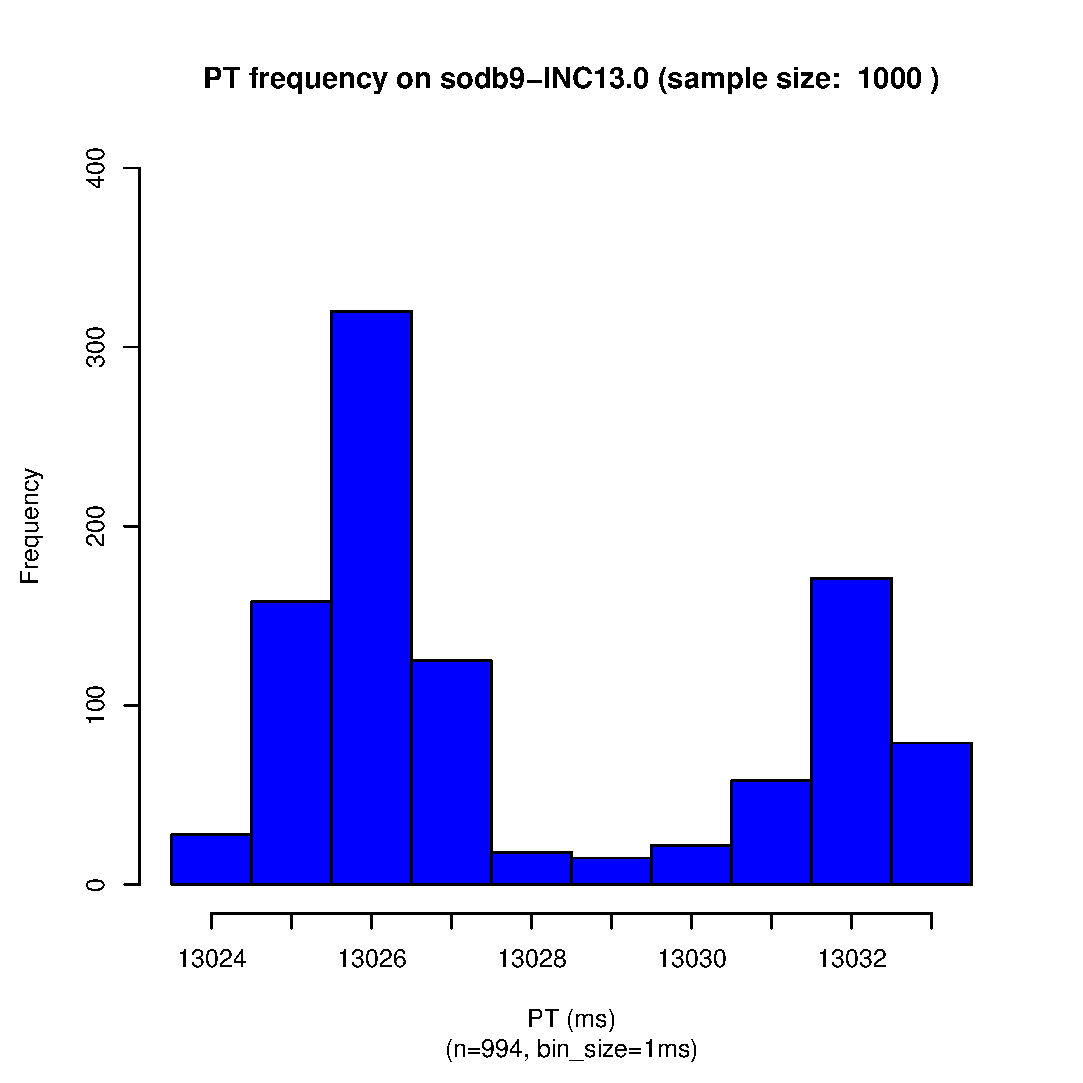
\includegraphics[scale=0.43]{sodb9_INC13_0_dist.eps}
		\label{fig:s9_inc13_dist}
	}
	\subfigure[PT frequency on INC13]{
		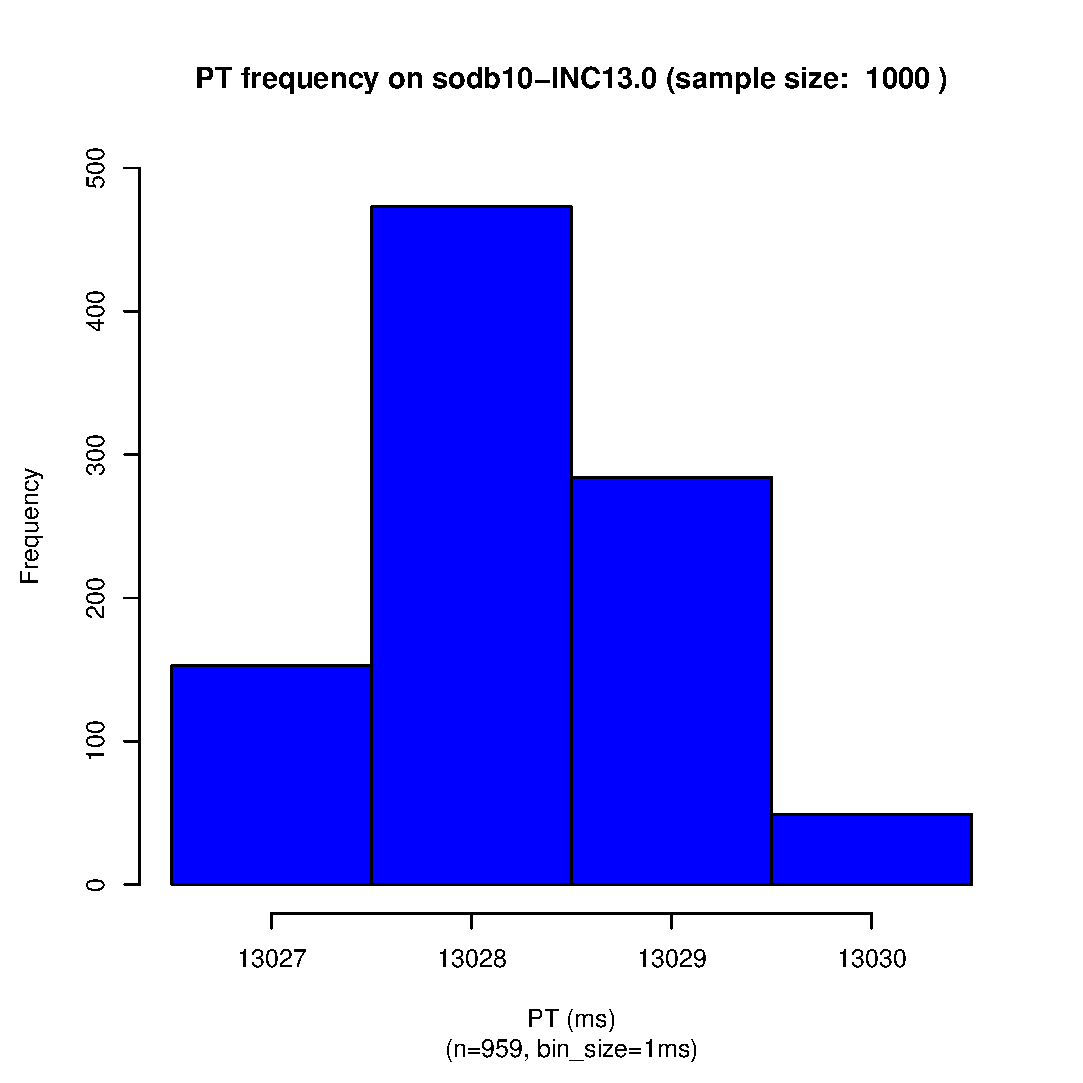
\includegraphics[scale=0.43]{sodb10_INC13_0_dist.eps}
		\label{fig:s10_inc13_dist}
	}	
	\subfigure[PT frequency on INC13]{
		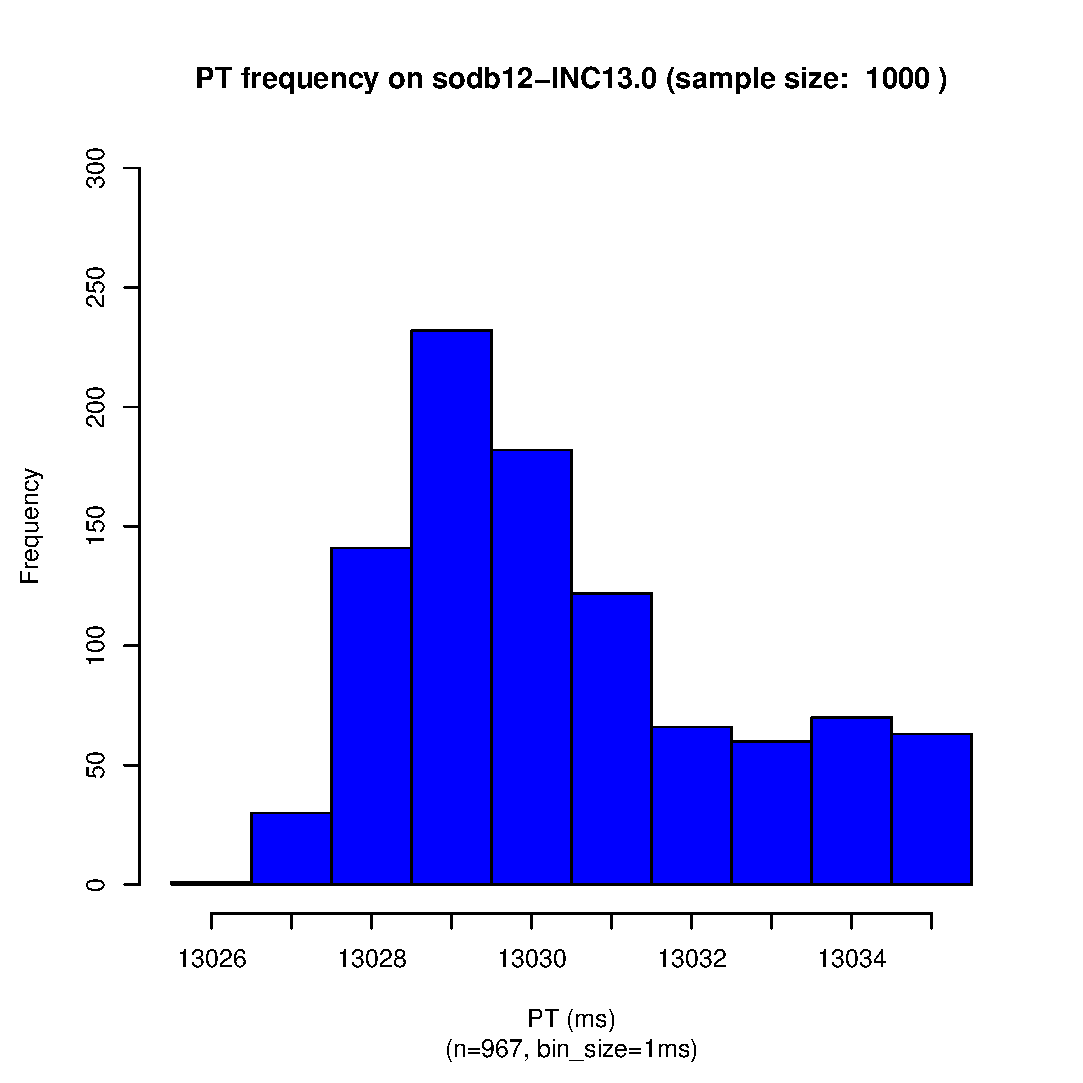
\includegraphics[scale=0.43]{sodb12_INC13_0_dist.eps}
		\label{fig:s12_inc13_dist}
	}
	\caption{PT Histograms on INC13~\label{fig:dm_2}}
\end{figure}

\newpage
\clearpage

\begin{figure}[h]
	\centering
	\subfigure[PT frequency on INC17.2]{
		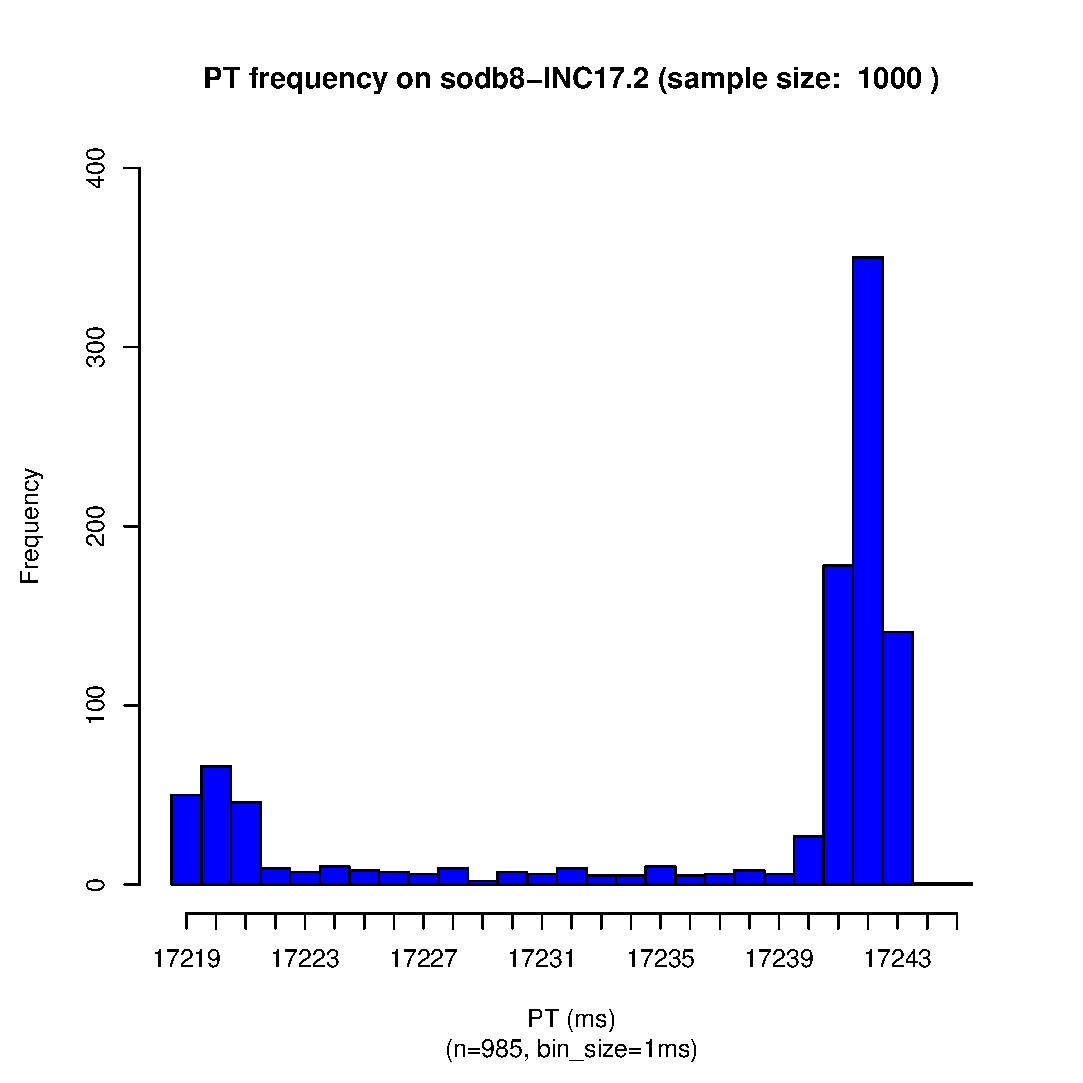
\includegraphics[scale=0.43]{sodb8_INC17_2_dist.eps}
		\label{fig:s8_inc17_2_dist}
	}	
	\subfigure[PT frequency on INC17.2]{
		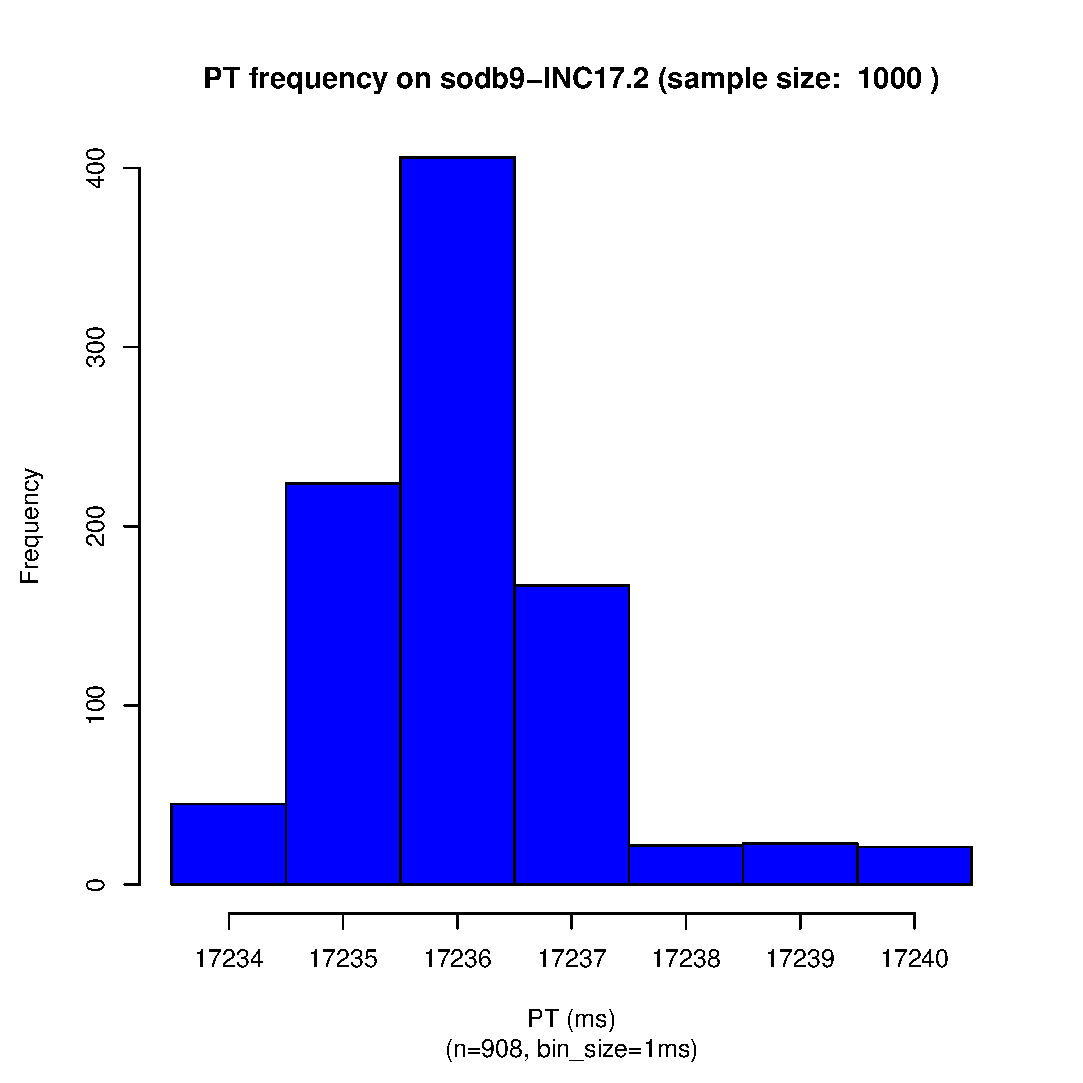
\includegraphics[scale=0.43]{sodb9_INC17_2_dist.eps}
		\label{fig:s9_inc17_2_dist}
	}
	\subfigure[PT frequency on INC17.2]{
		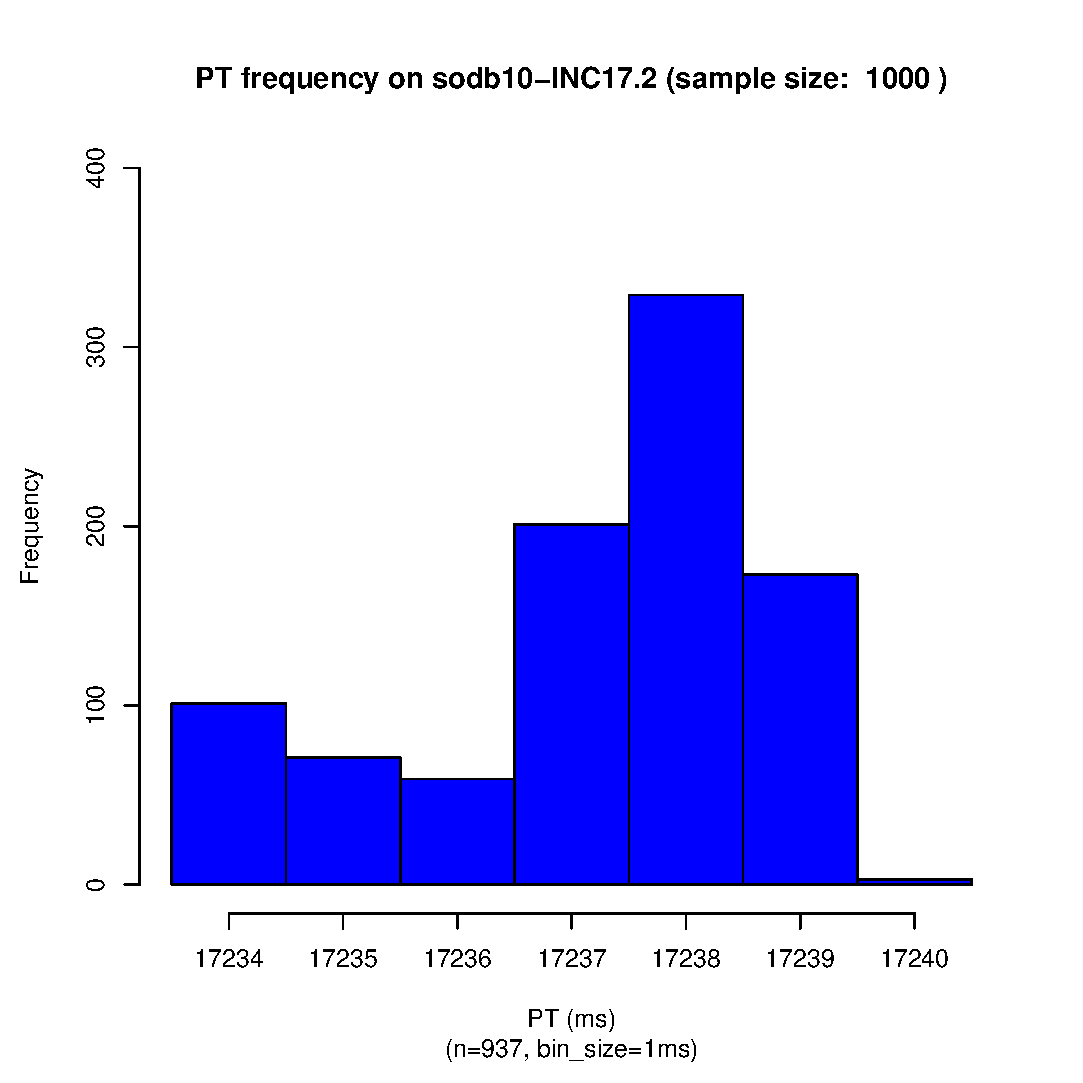
\includegraphics[scale=0.43]{sodb10_INC17_2_dist.eps}
		\label{fig:s10_inc17_2_dist}
	}	
	\subfigure[PT frequency on INC17.2]{
		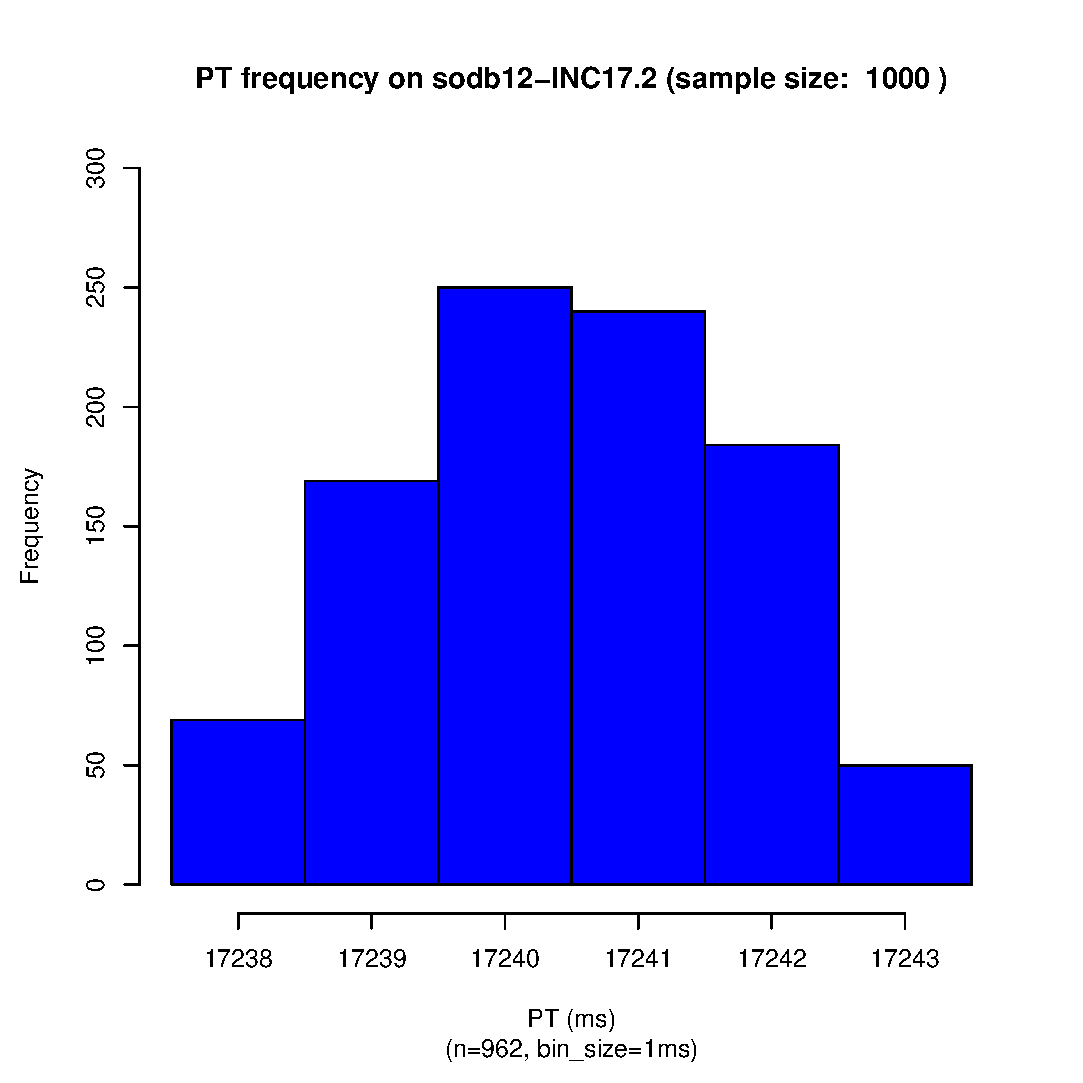
\includegraphics[scale=0.43]{sodb12_INC17_2_dist.eps}
		\label{fig:s12_inc17_2_dist}
	}
	\caption{PT Histograms on INC17.2~\label{fig:dm_3}}
\end{figure}

\newpage
\clearpage

\subsection{One-to-One Comparison between An Insertion Sort \& A Corresponding INC Programs~\label{sec:sort}} 
This section compares program time histograms 
of insertion sort and INC (a nested-for-loop) programs. 
The insertion sort program 
sorts the elements of a given array in non-decreasing order.  
The program repeatedly runs 300 times for a given input size. 
The input size for the program varies from 144K to 344K integer elements, which are randomly generated. 
Note that each sort program over a specific input size is termed SORT{\it x}: 
for instance, SORT100 indicates the insertion sort program over 100K elements. 
An INC program's task length is correspondingly determined by the program time 
of an SORT program. In Figures~\ref{fig:sort1},~\ref{fig:sort2}, and~\ref{fig:sort3} 
we perform a match on an SORT program and its corresponding INC program.

%
%Figures~\ref{fig:sort1} and ~\ref{fig:sort2} exhibit 
%histograms of the execution times measured on the same insertion sort program as 
%the input size grows from 100K to 1,160K elements.% by the steps of 2x. 
%Note that we used one standard deviation in Figure~\ref{fig:sort400_dist} as
%a couple of outliers, which were not eliminated by the original protocol, 
%resulted in disturbing the rendering of a clean distribution. 

\begin{figure}[h]
	\centering
	\subfigure[PT frequency on SORT144]{
		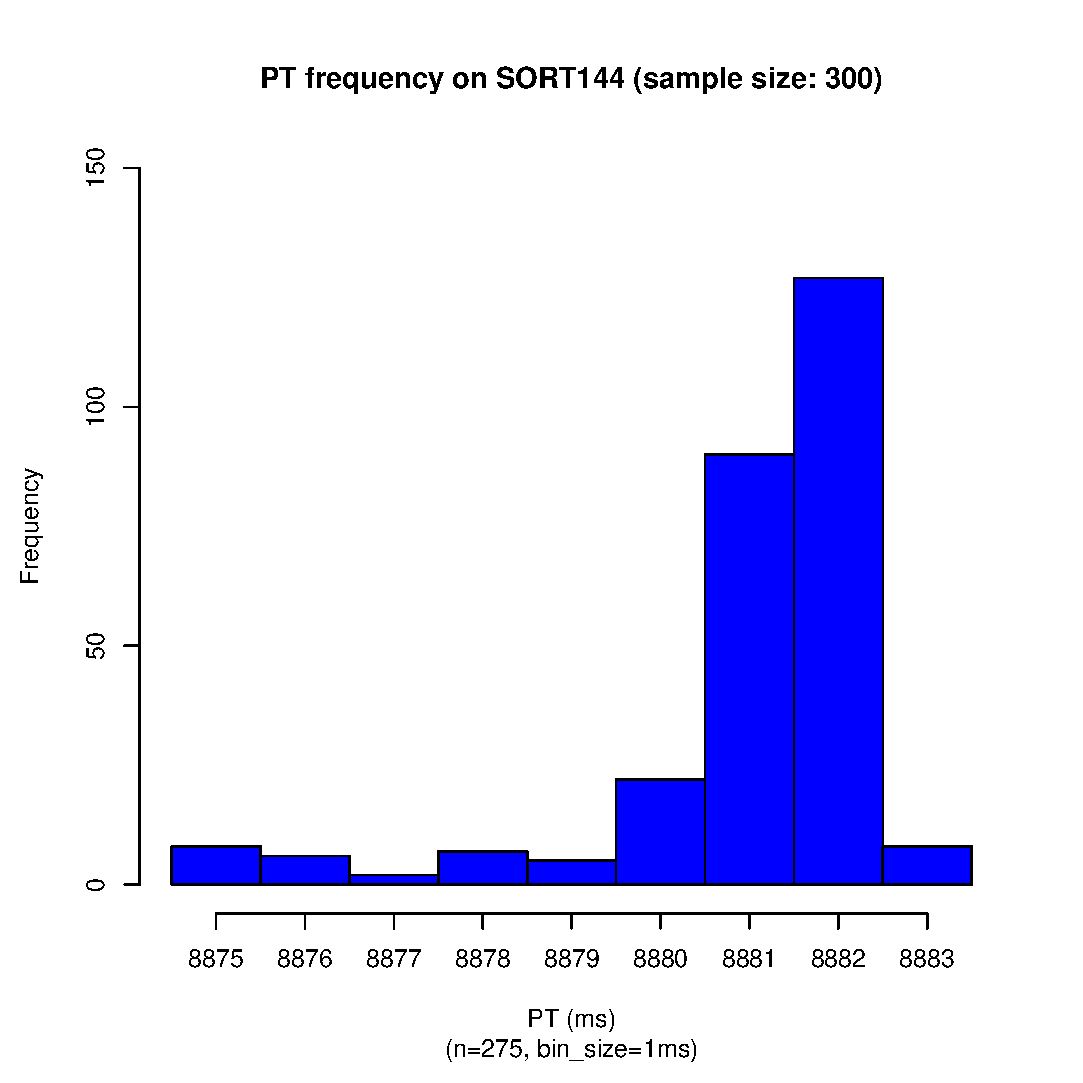
\includegraphics[scale=0.43]{sort144_dist.eps}
		\label{fig:sort144_dist}
	}	
	\subfigure[PT frequency on INC8.8]{
		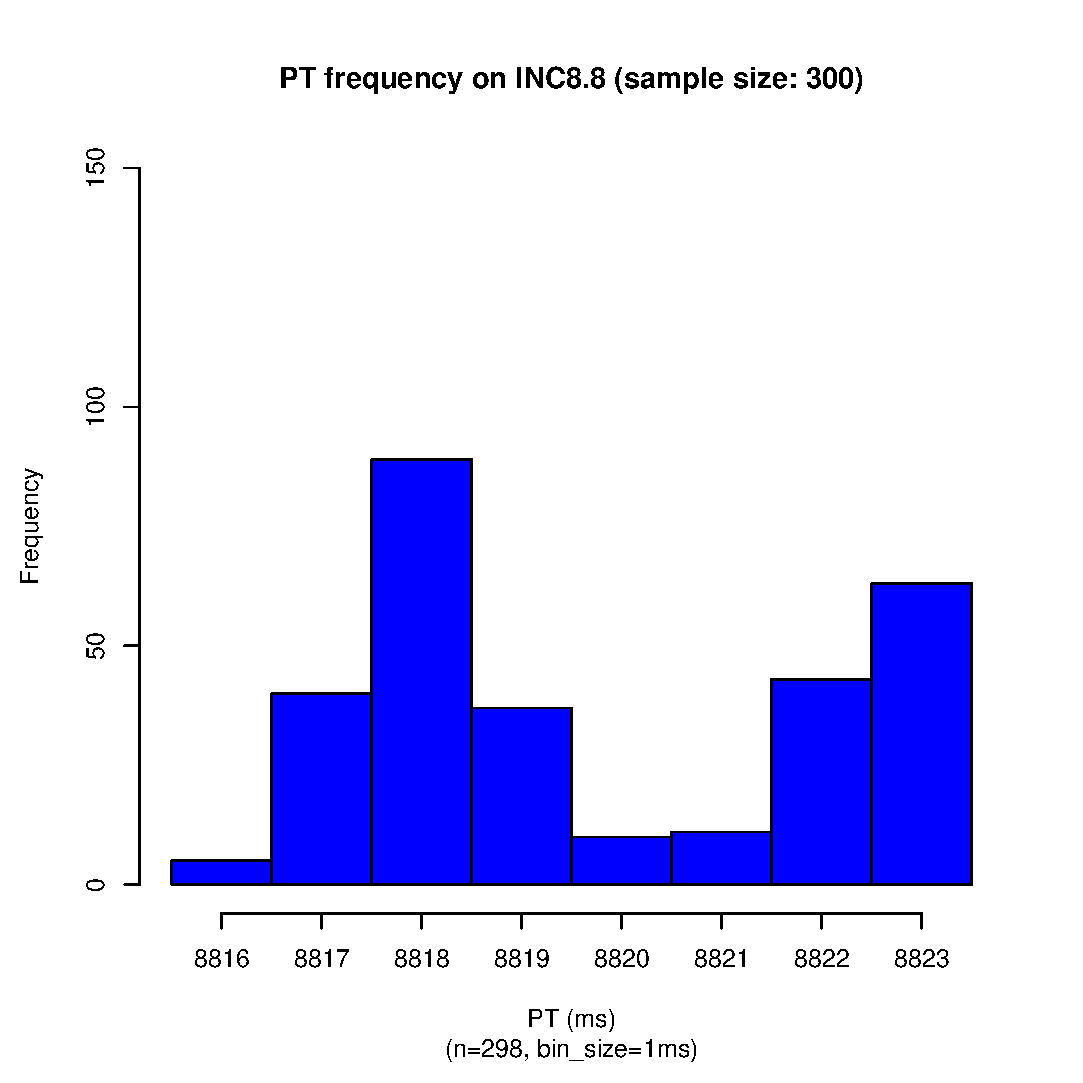
\includegraphics[scale=0.43]{inc8.8_dist.eps}
		\label{fig:inc8.8_dist}
	}
	\subfigure[PT frequency on SORT177]{
		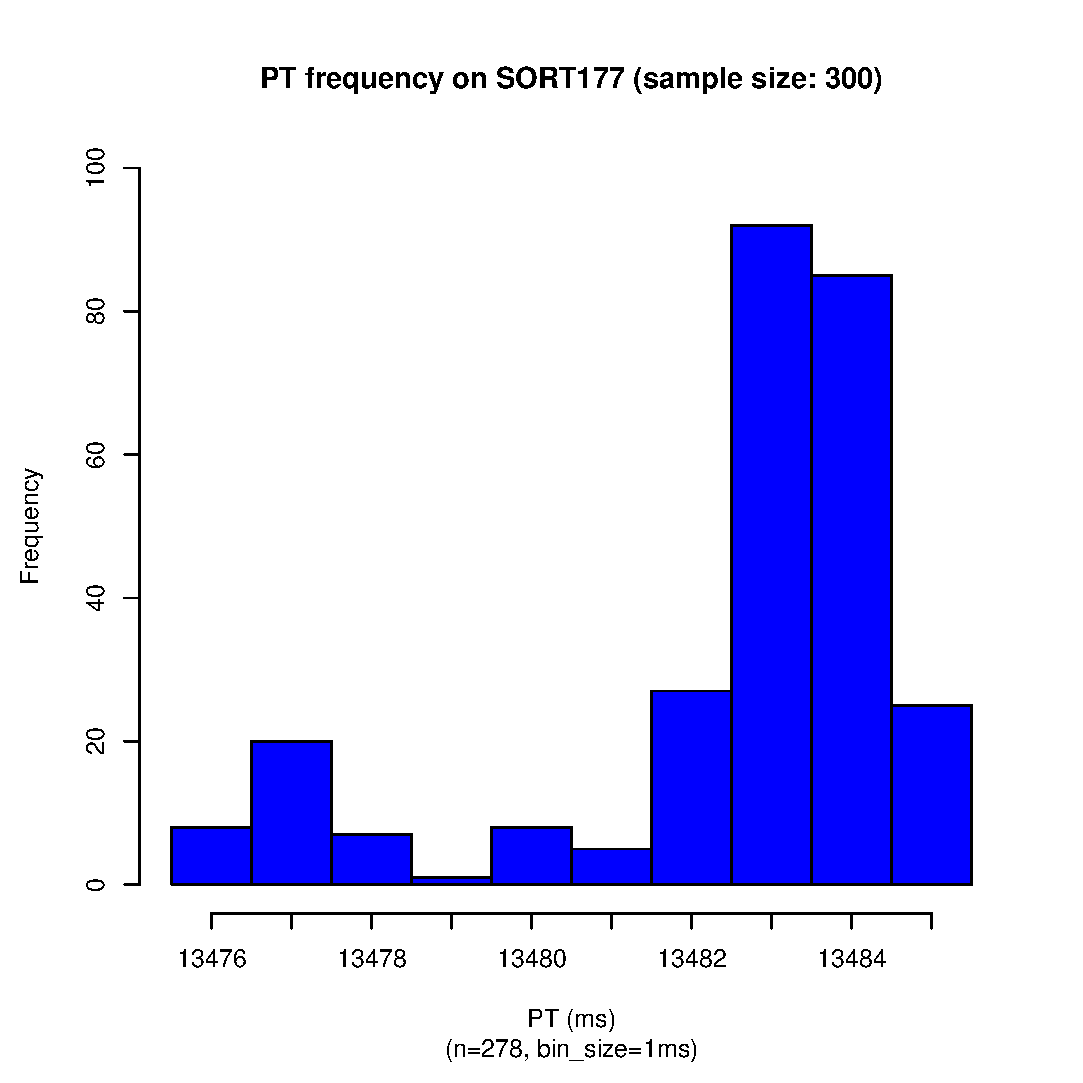
\includegraphics[scale=0.43]{sort177_dist.eps}
		\label{fig:sort177_dist}
	}	
	\subfigure[PT frequency on INC13]{
		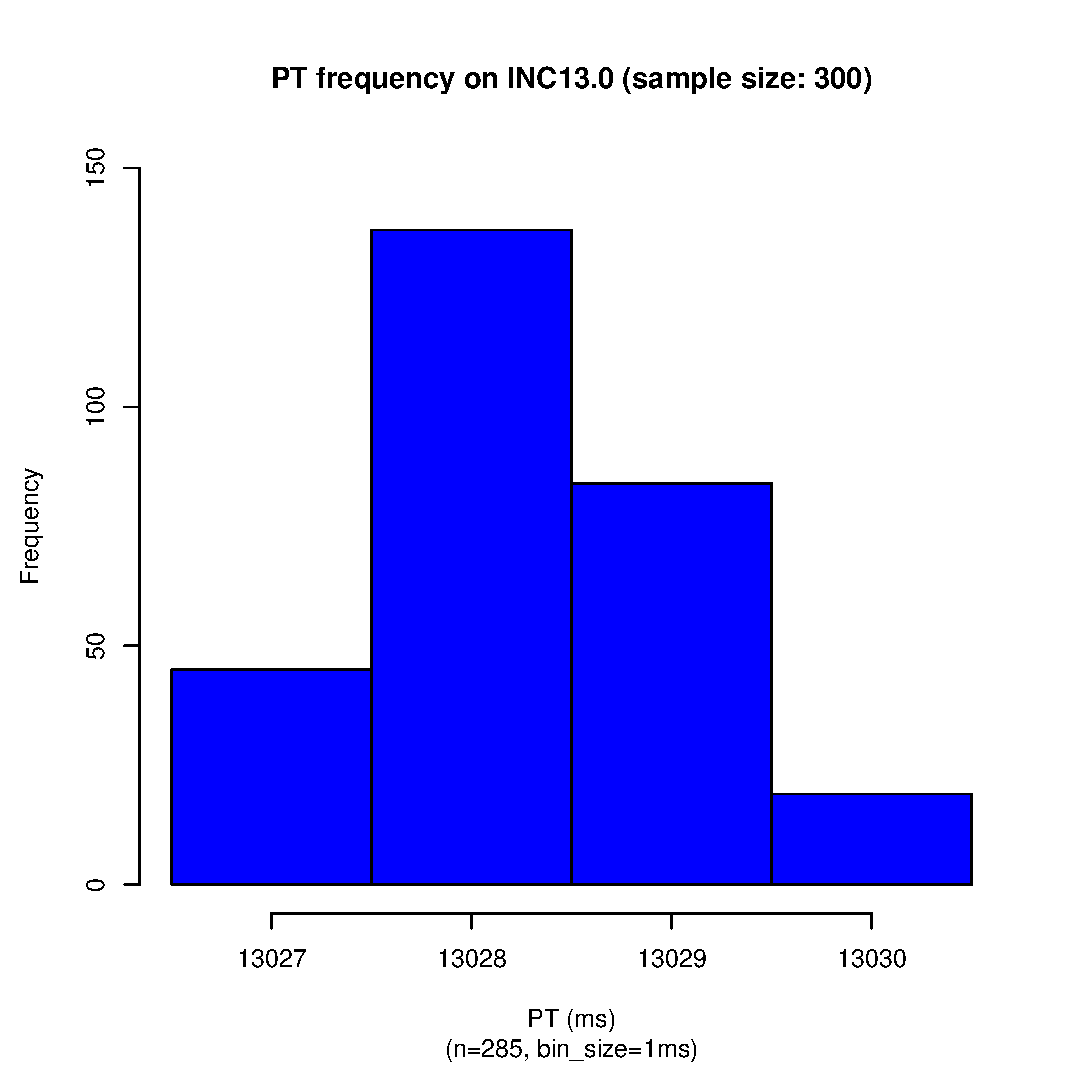
\includegraphics[scale=0.43]{inc13.0_dist.eps}
		\label{fig:inc13_dist}
	}
	\caption{PT Histograms I~\label{fig:sort1}}
\end{figure}

\begin{figure}[h]
	\centering
	\subfigure[PT frequency on SORT144]{
		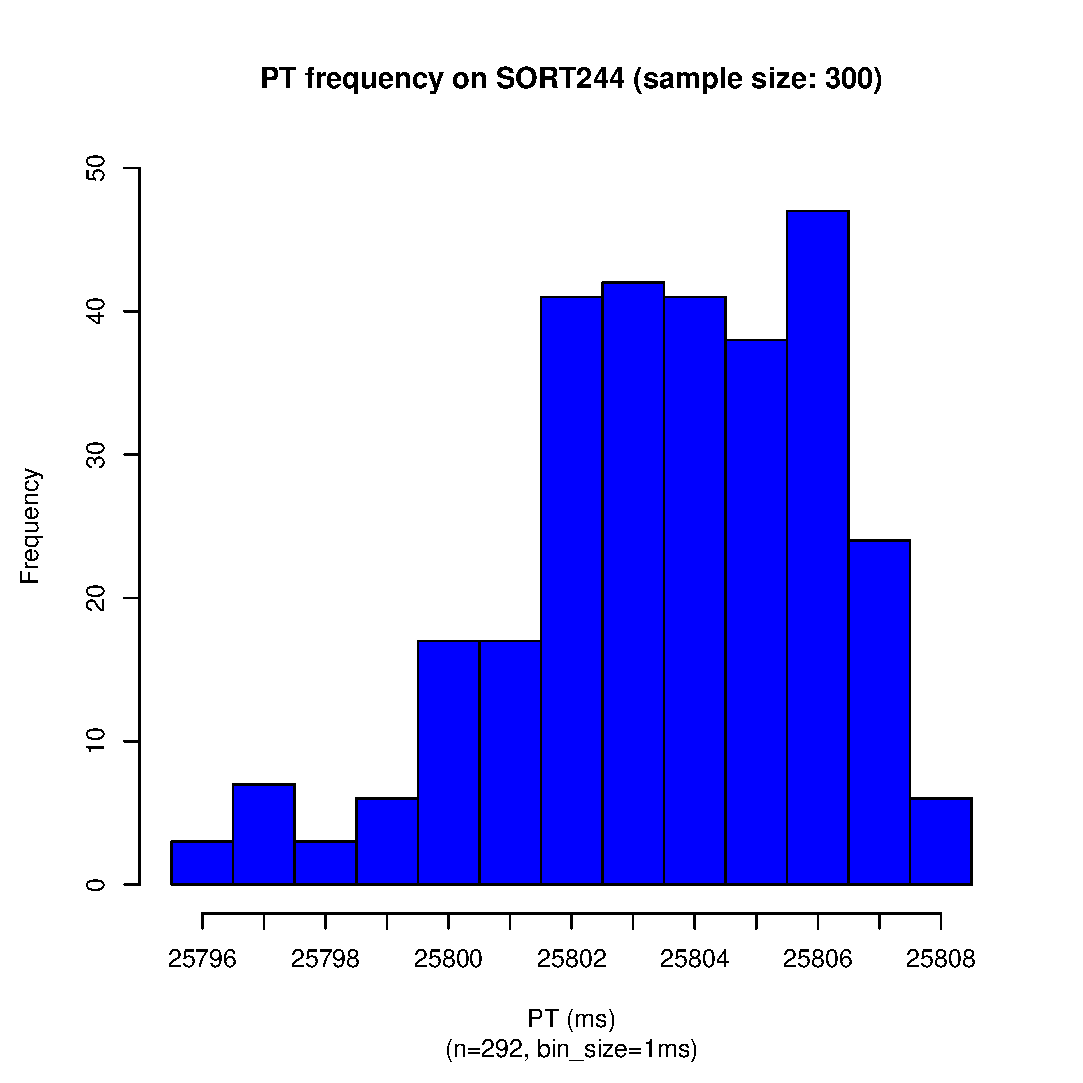
\includegraphics[scale=0.43]{sort244_dist.eps}
		\label{fig:sort144_dist}
	}	
	\subfigure[PT frequency on INC25.8]{
		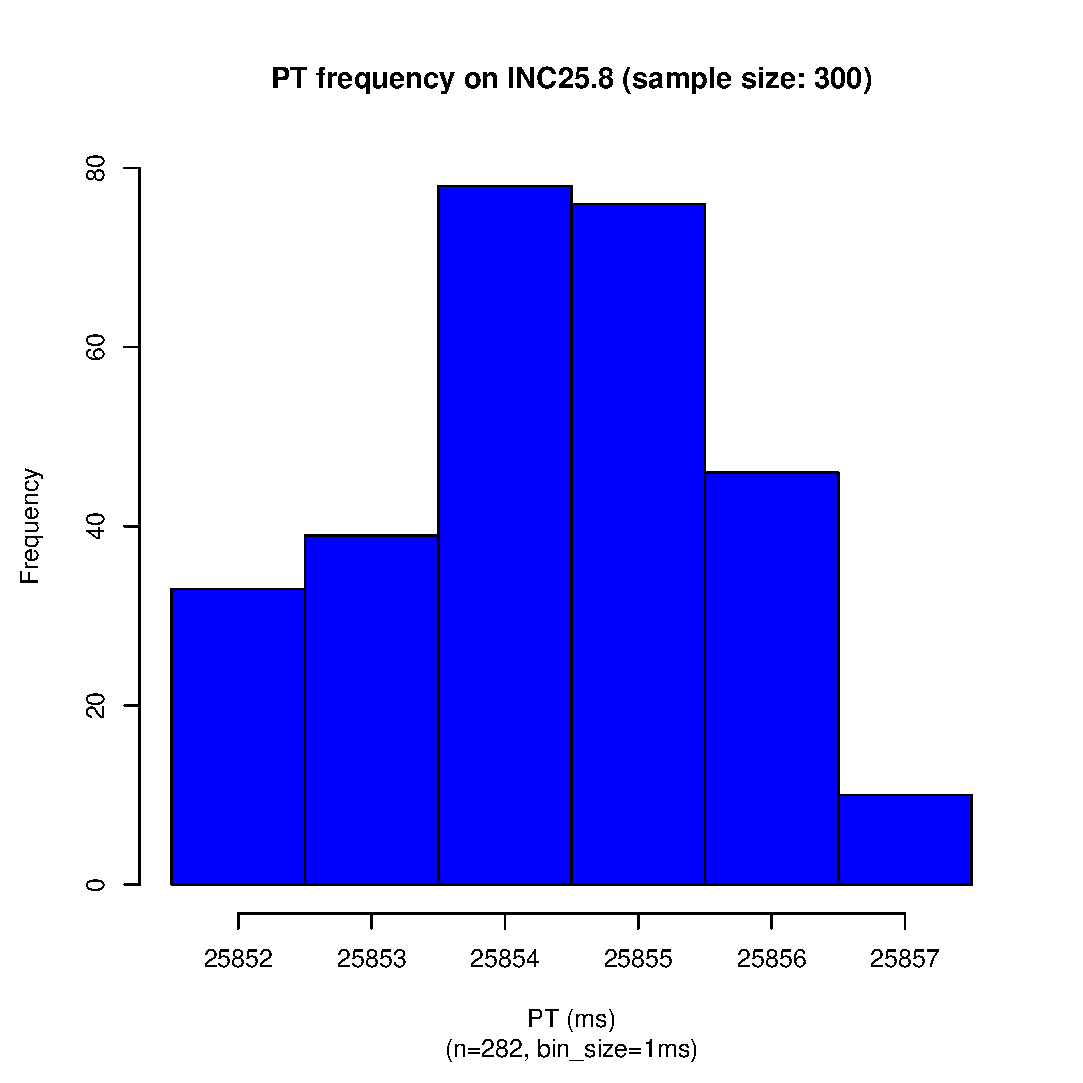
\includegraphics[scale=0.43]{inc25.8_dist.eps}
		\label{fig:inc25.8_dist}
	}
	\subfigure[PT frequency on SORT288]{
		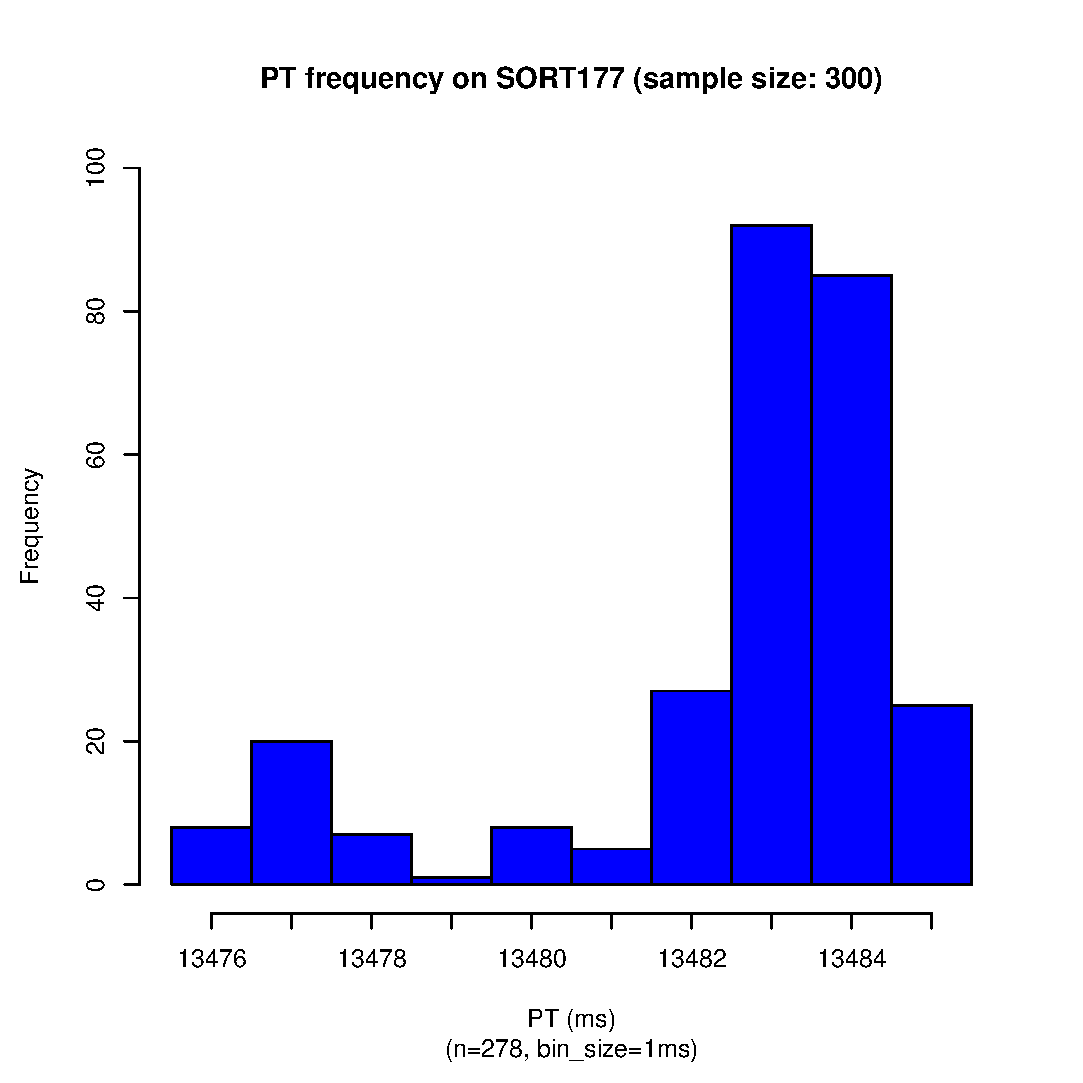
\includegraphics[scale=0.43]{sort177_dist.eps}
		\label{fig:sort177_dist}
	}	
	\subfigure[PT frequency on INC35]{
		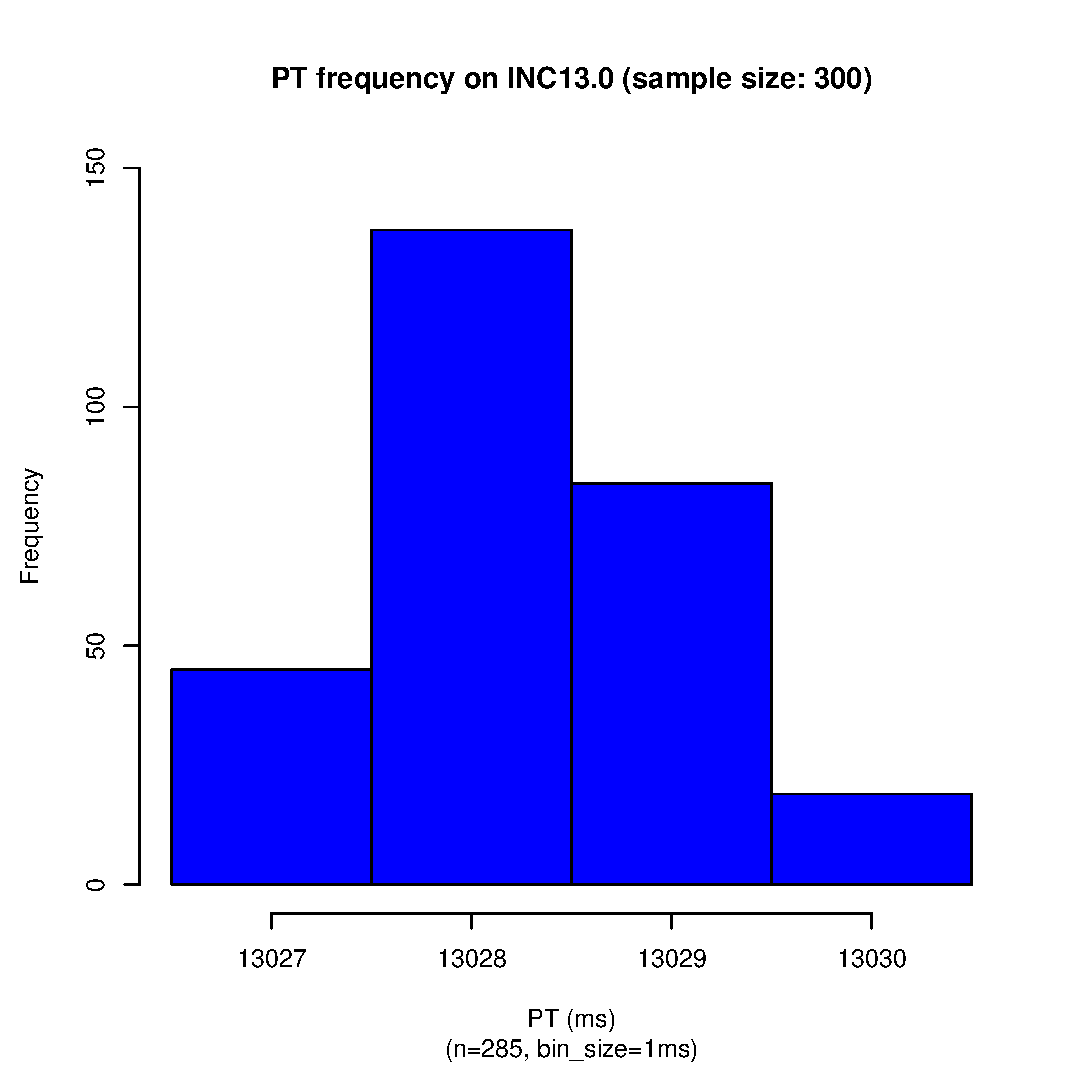
\includegraphics[scale=0.43]{inc13.0_dist.eps}
		\label{fig:inc35_dist}
	}
	\caption{PT Histogram Comparison II~\label{fig:sort2}}
\end{figure}

\begin{figure}[h]
	\centering
	\subfigure[PT frequency on SORT344]{
		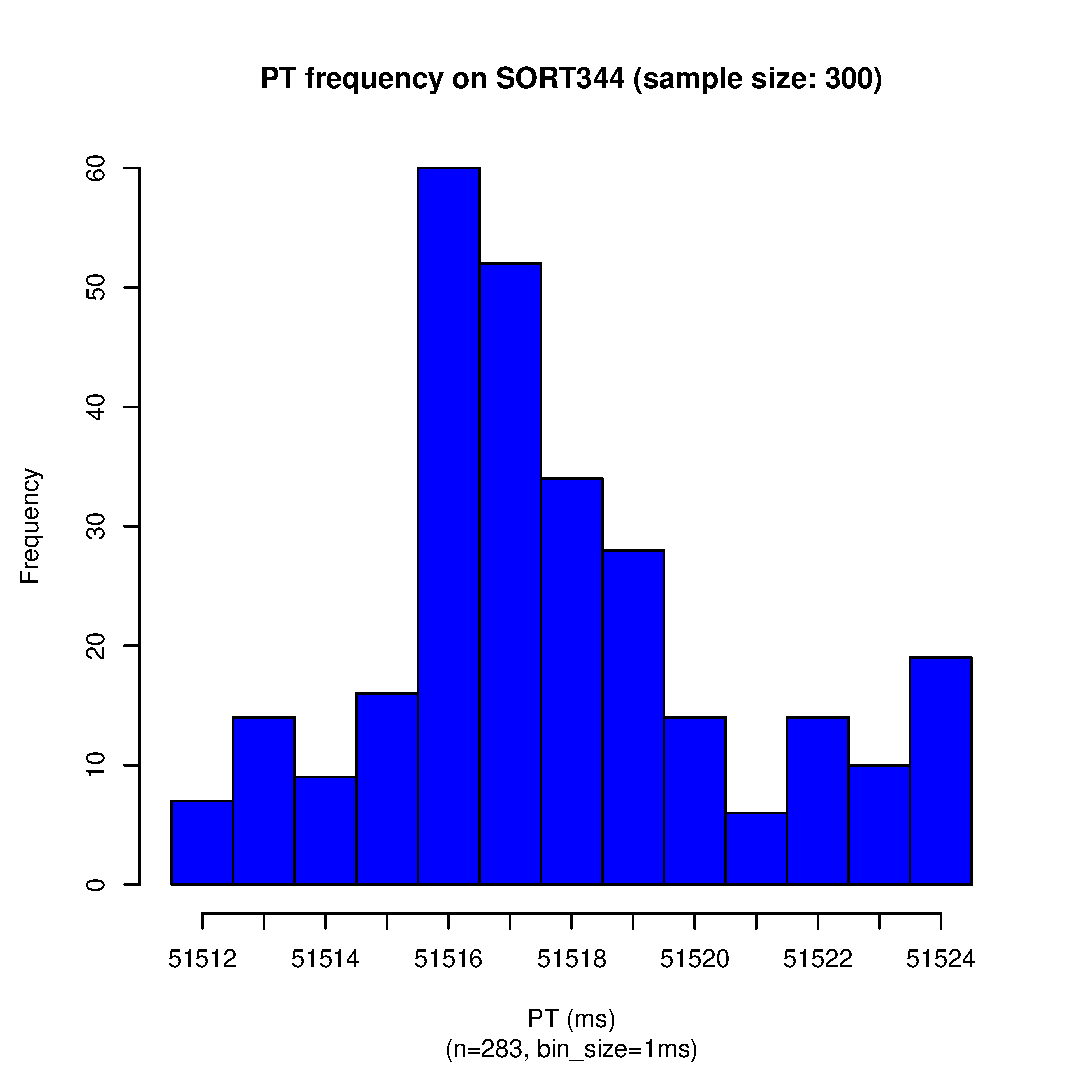
\includegraphics[scale=0.43]{sort344_dist.eps}
		\label{fig:sort344_dist}
	}	
	\subfigure[PT frequency on INC51.5]{
		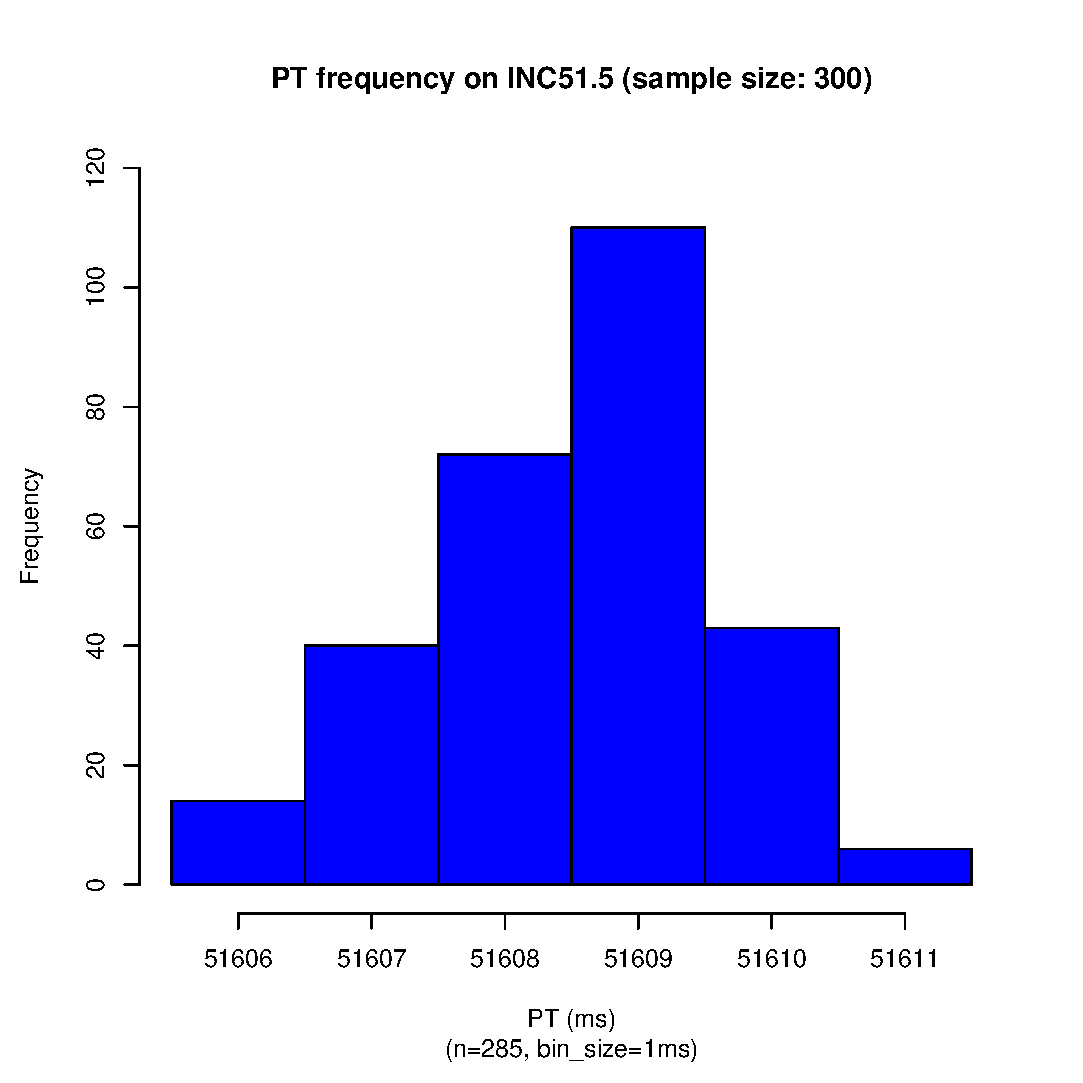
\includegraphics[scale=0.43]{inc51.5_dist.eps}
		\label{fig:inc51.5_dist}
	}
	\caption{PT Histogram Comparison III~\label{fig:sort3}}
\end{figure}

\clearpage
\pagebreak

\section{Additional Insertion Sort~\label{sec:add_new}} 

\begin{figure}[h]
	\centering
%	\subfigure[PT frequency on SORT25]{
%		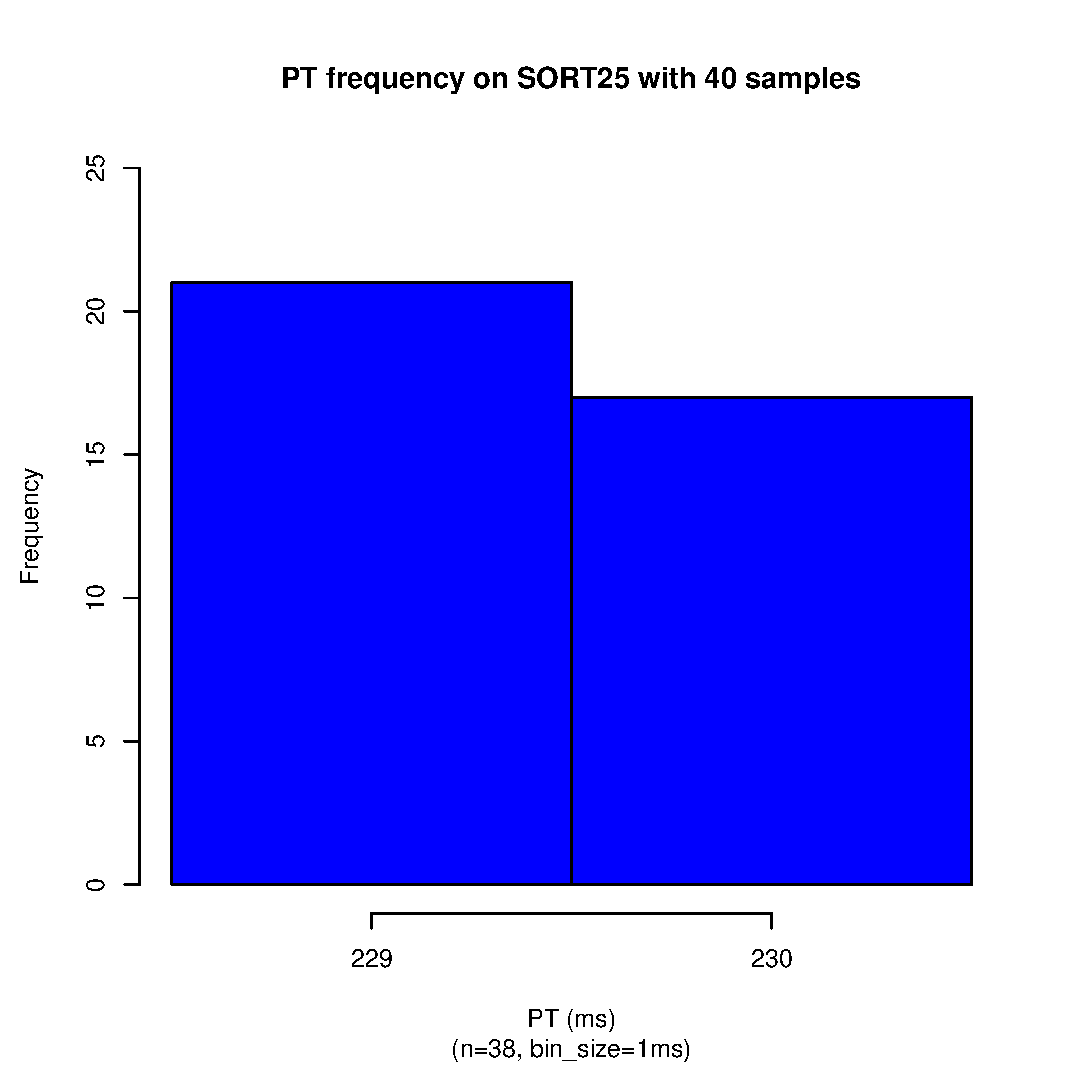
\includegraphics[scale=0.43]{sort25_dist.eps}
%		\label{fig:sort25_dist}
%	}
%	\subfigure[PT frequency on SORT50]{
%		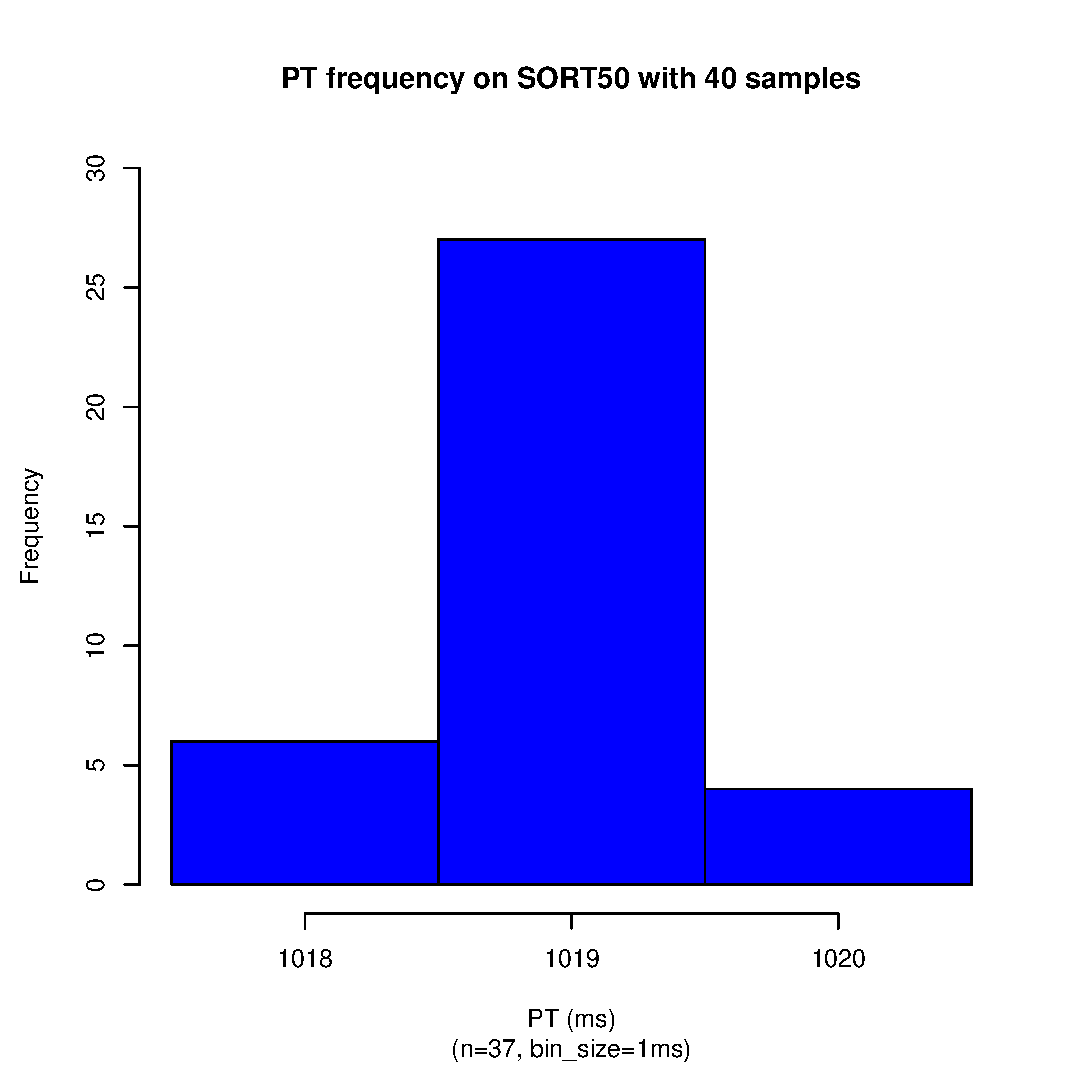
\includegraphics[scale=0.43]{sort50_dist.eps}
%		\label{fig:sort50_dist}
%	}
	\subfigure[PT frequency on SORT100]{
		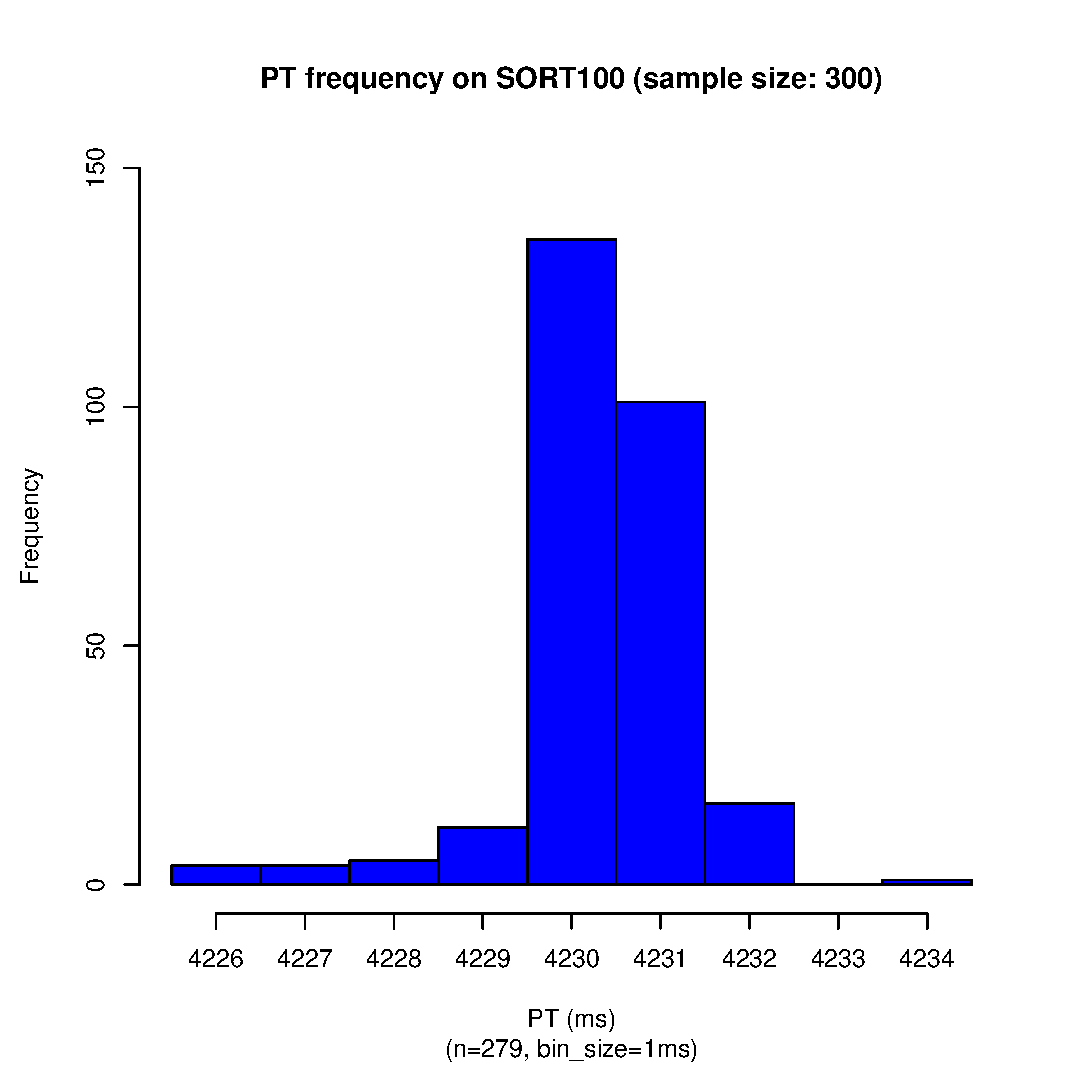
\includegraphics[scale=0.43]{sort100_dist.eps}
		\label{fig:sort100_dist}
	}
	\subfigure[PT frequency on SORT400]{
		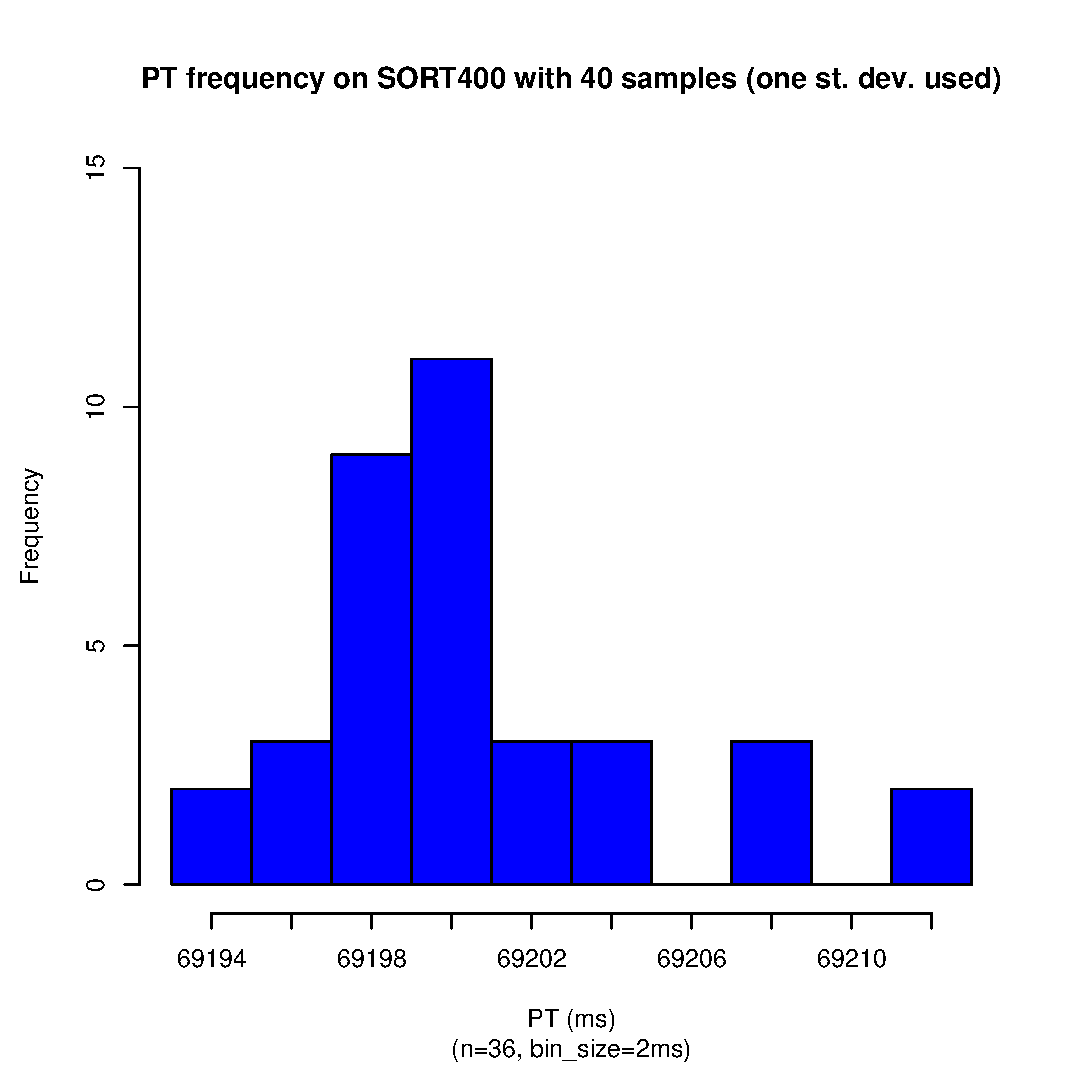
\includegraphics[scale=0.43]{sort400_dist.eps}
		\label{fig:sort400_dist}
	}
	\subfigure[PT frequency on SORT580]{
		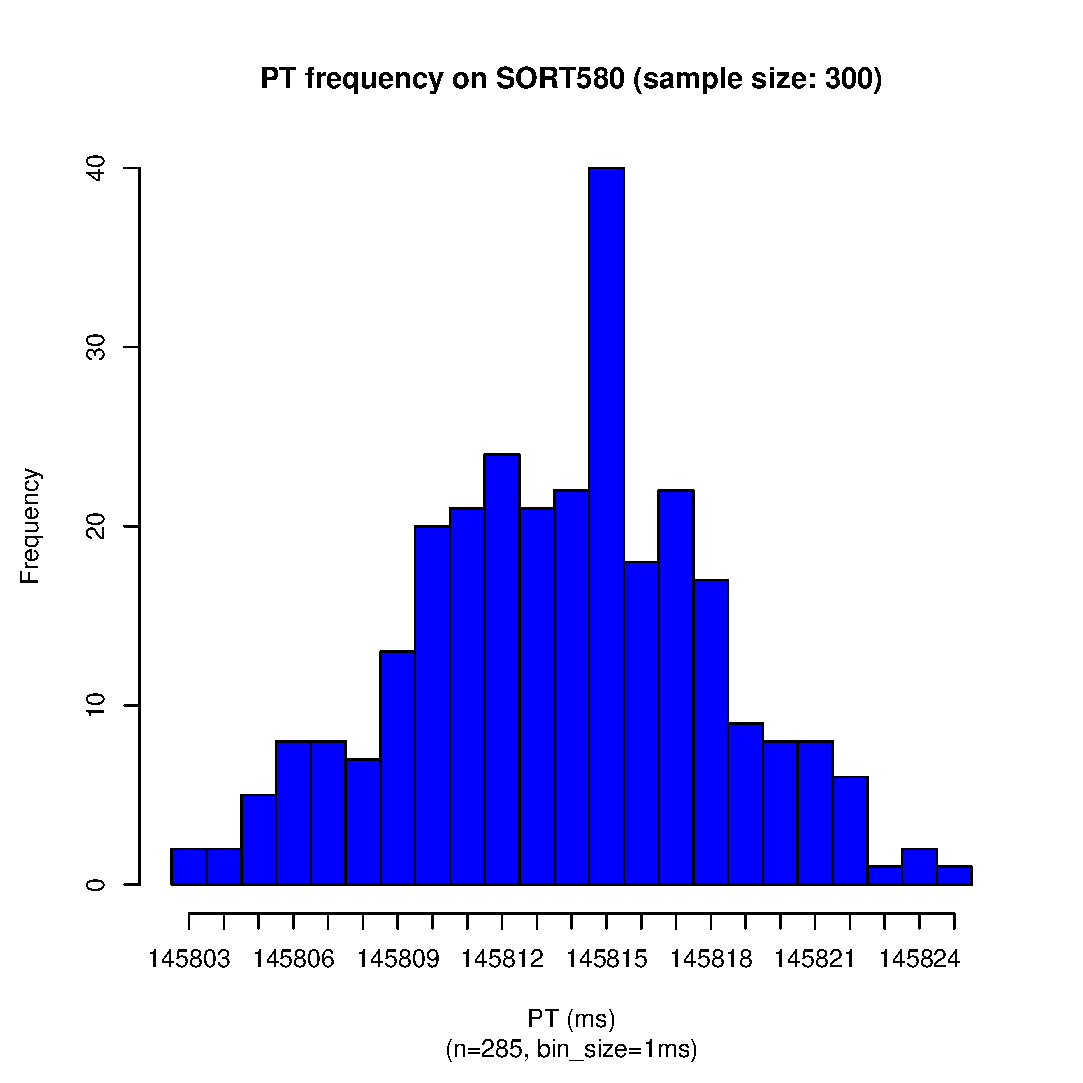
\includegraphics[scale=0.43]{sort580_dist.eps}
		\label{fig:sort588_dist}
	}
	\caption{PT Histograms of SORT100 ... SORT580~\label{fig:n_sort1}}
\end{figure}

\clearpage
\pagebreak

\begin{figure}[h]
	\centering
	\subfigure[PT frequency on SORT800]{
		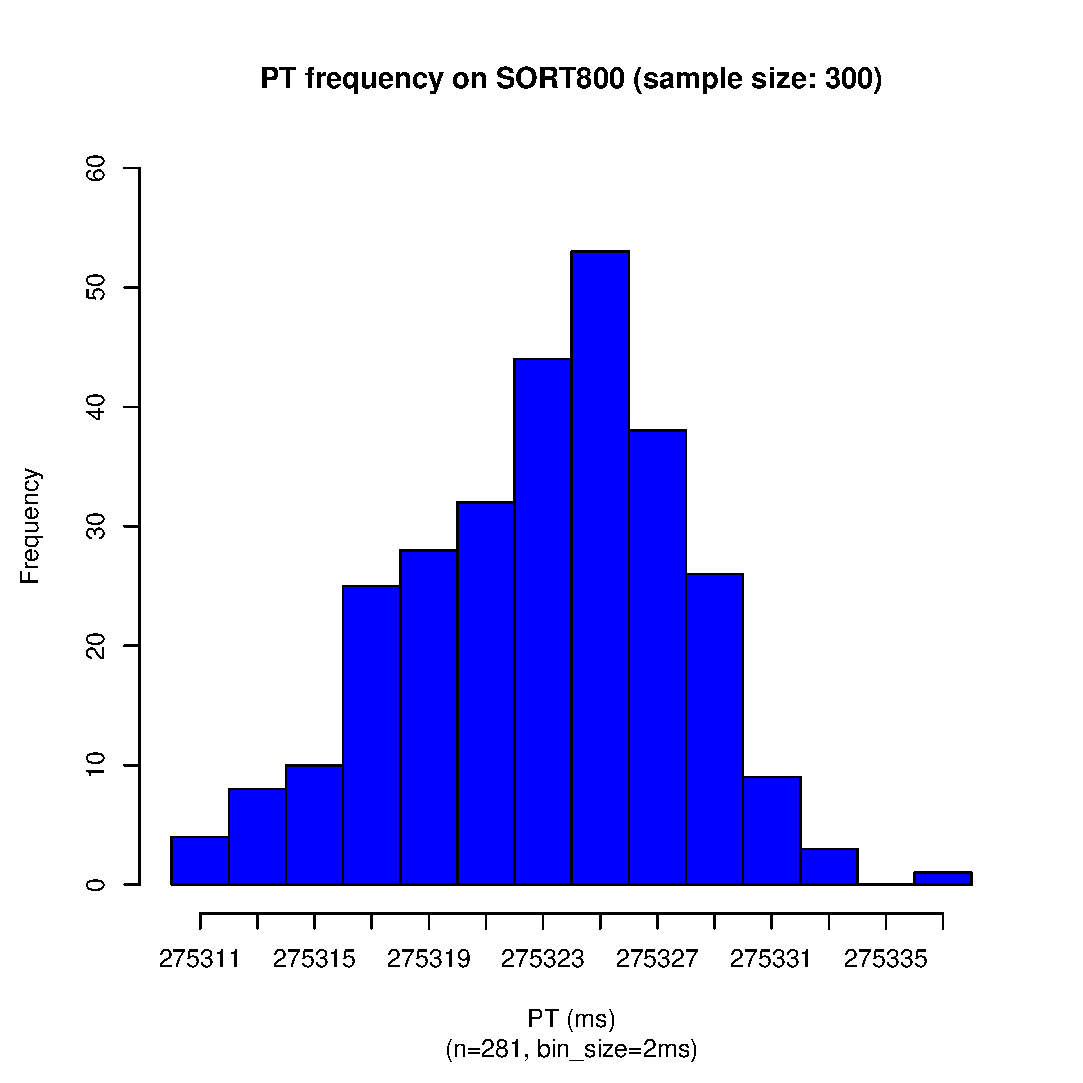
\includegraphics[scale=0.43]{sort800_dist.eps}
		\label{fig:sort800_dist}
	}
	\subfigure[PT frequency on SORT1000]{
		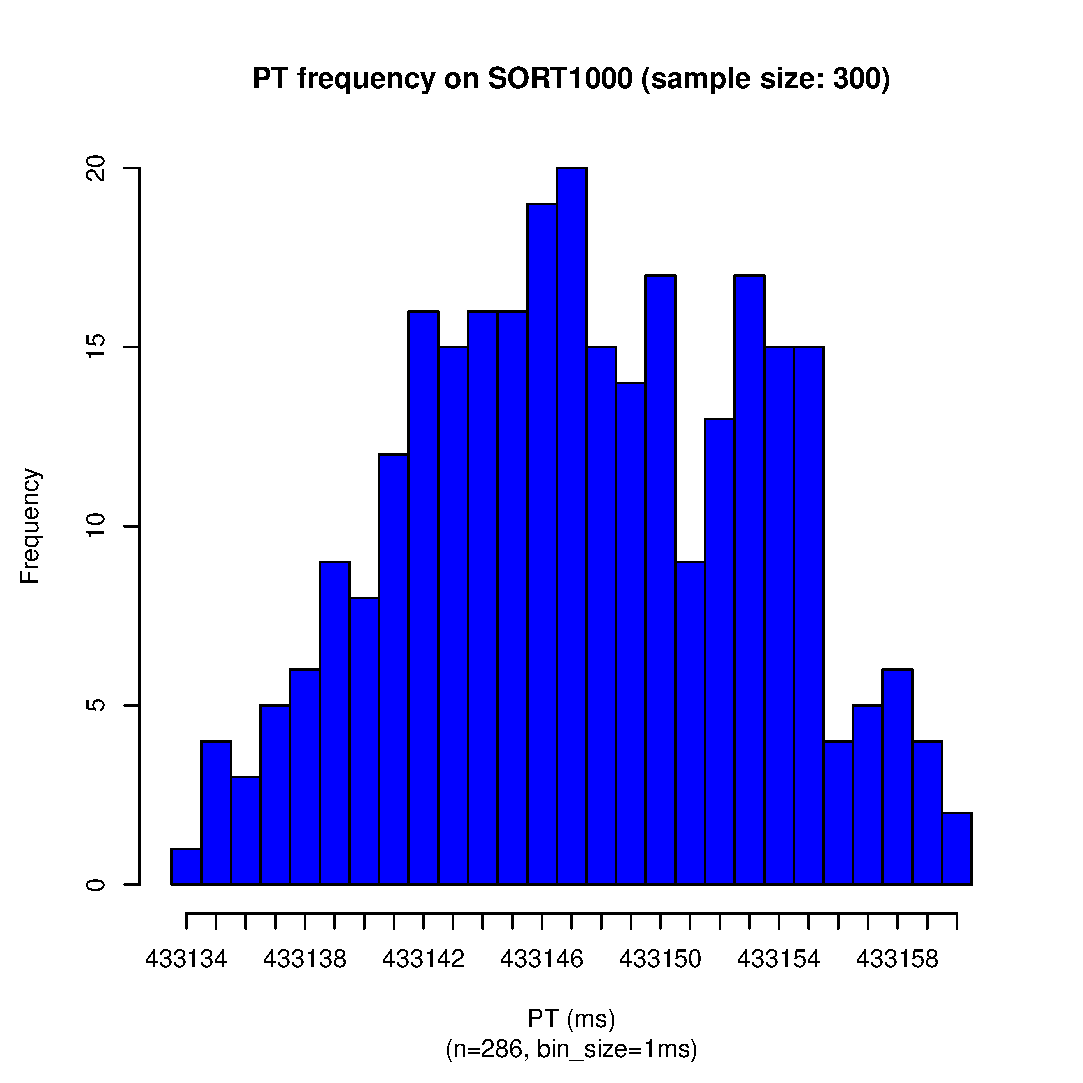
\includegraphics[scale=0.43]{sort1000_dist.eps}
		\label{fig:sort1000_dist}
	}
	\subfigure[PT frequency on SORT1160]{
		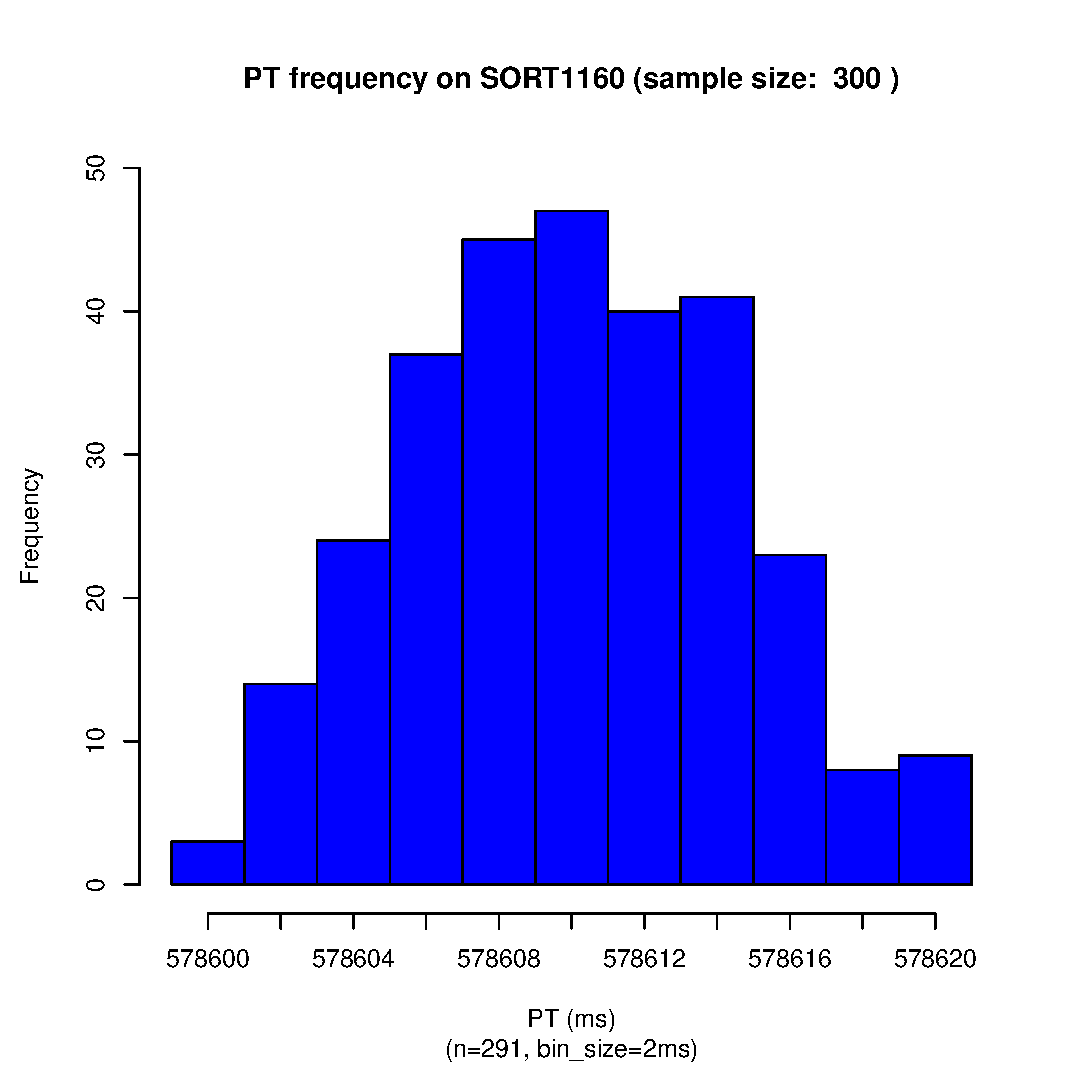
\includegraphics[scale=0.43]{sort1160_dist.eps}
		\label{fig:sort1160_dist}
	}
	\subfigure[PT frequency on SORT2320 (not complete)]{
		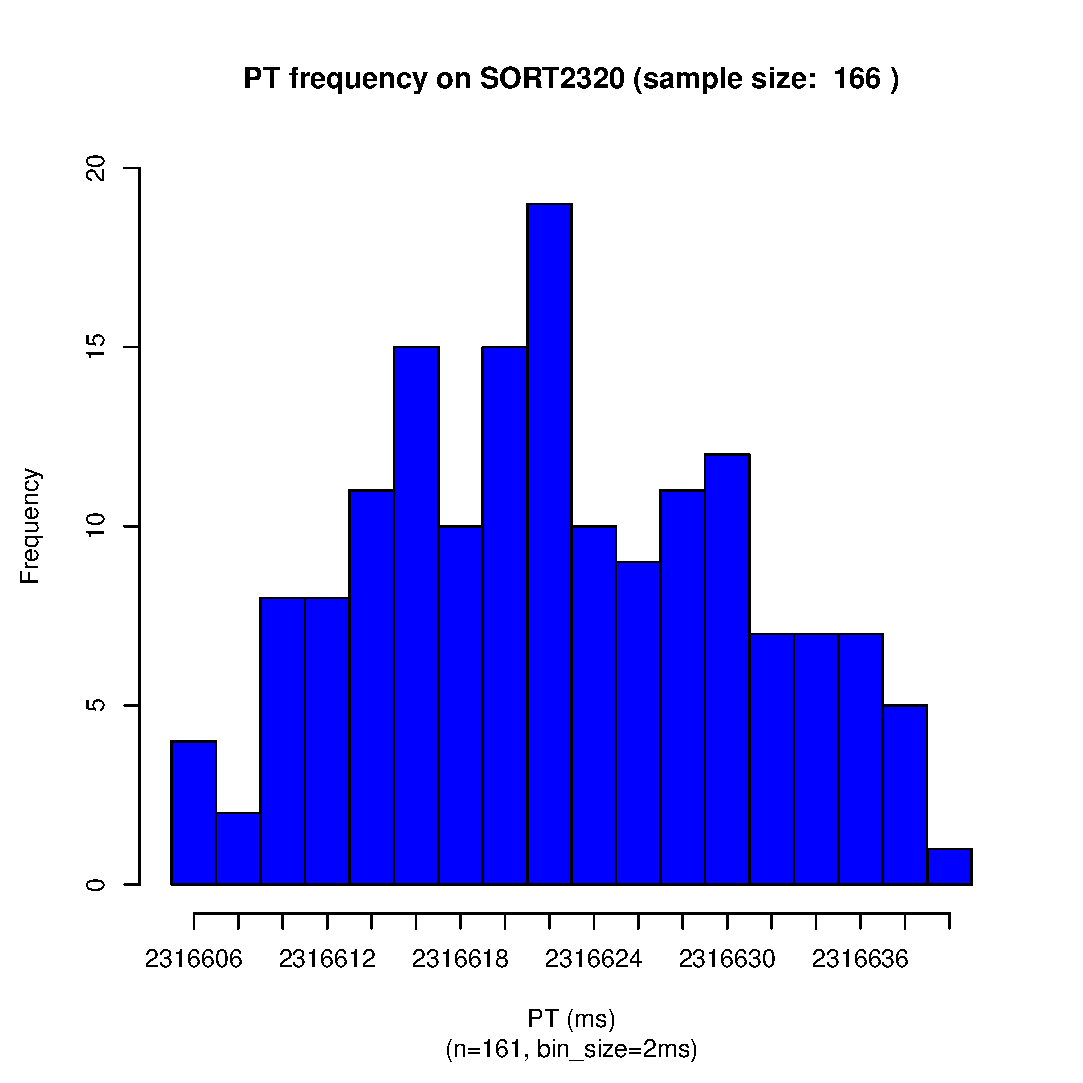
\includegraphics[scale=0.43]{sort2320_dist.eps}
		\label{fig:sort2320_dist}
	}
	\caption{PT Histograms of SORT800 ... SORT2320~\label{fig:n_sort2}}
\end{figure}

%\subsection{Insertion sort~\label{sec:sort}} 
%This section shows a series of histograms of an insertion sorting program that 
%sorts the elements of a given array in non-decreasing order. 
%The program repeatedly runs 300 times for a given input size. 
%The input size for the program 
%varies from 100,000 to 1,160,000 integer elements, which are randomly generated. 
%Note that each sort program over a specific input size is termed SORT{\it x}: 
%for instance, SORT100 indicates the insertion sort program over 100K elements. 
%
%Figures~\ref{fig:sort1} and ~\ref{fig:sort2} exhibit 
%histograms of the execution times measured on the same insertion sort program as 
%the input size grows from 100K to 1,160K elements.% by the steps of 2x. 
%Note that we used one standard deviation in Figure~\ref{fig:sort400_dist} as
%a couple of outliers, which were not eliminated by the original protocol, 
%resulted in disturbing the rendering of a clean distribution. 
%
%\begin{figure}[h]
%	\centering
%%	\subfigure[PT frequency on SORT25]{
%%		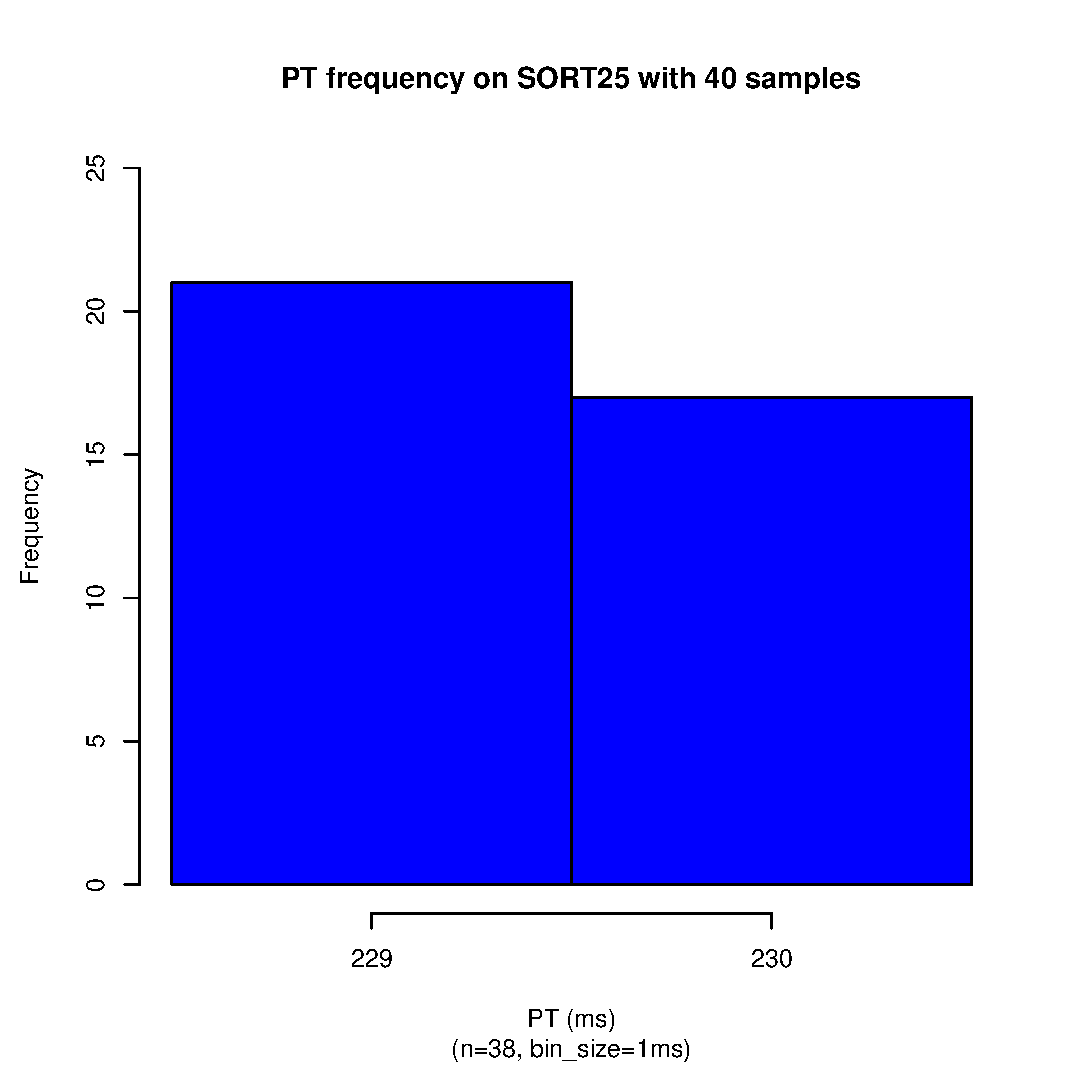
\includegraphics[scale=0.43]{sort25_dist.eps}
%%		\label{fig:sort25_dist}
%%	}
%%	\subfigure[PT frequency on SORT50]{
%%		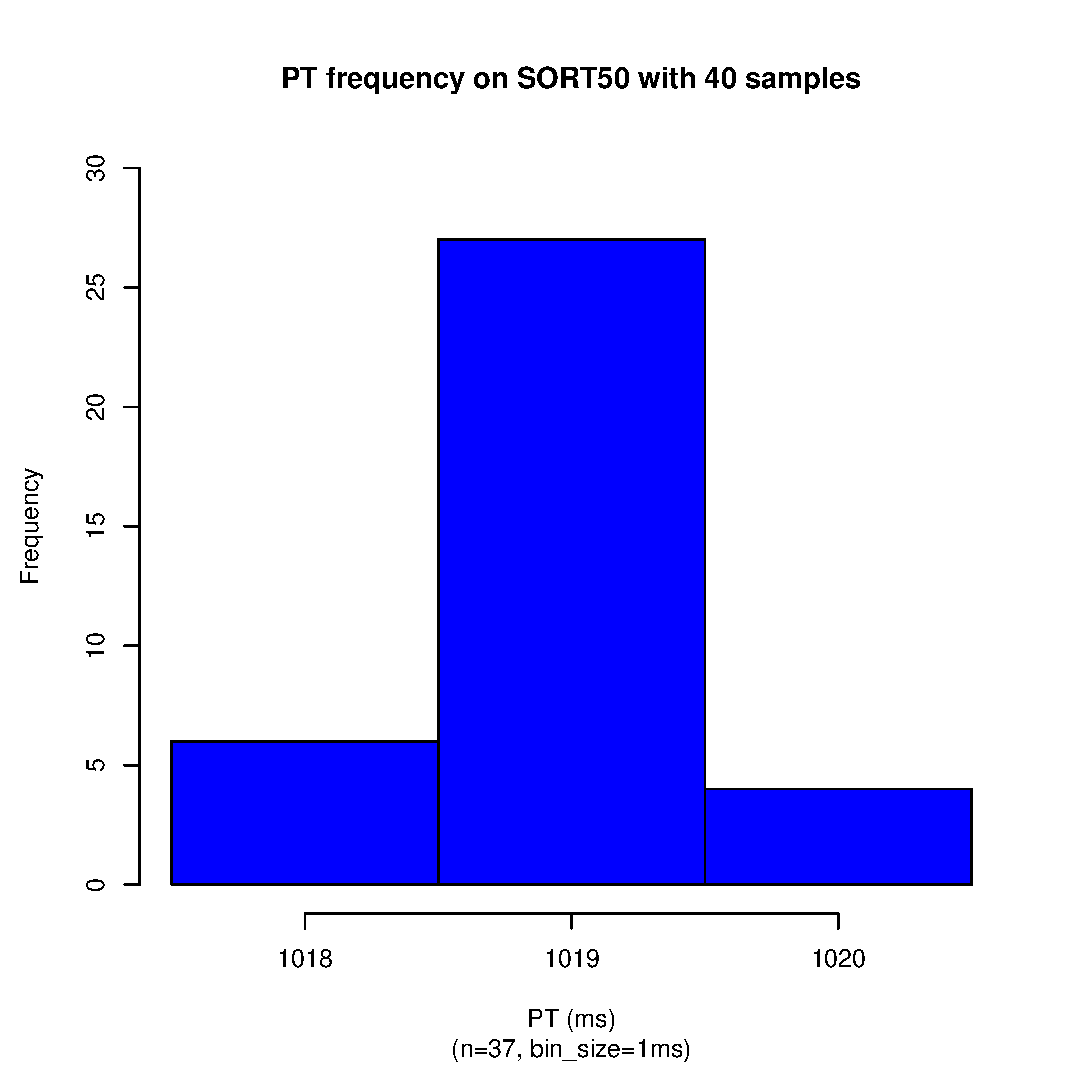
\includegraphics[scale=0.43]{sort50_dist.eps}
%%		\label{fig:sort50_dist}
%%	}
%	\subfigure[PT frequency on SORT100]{
%		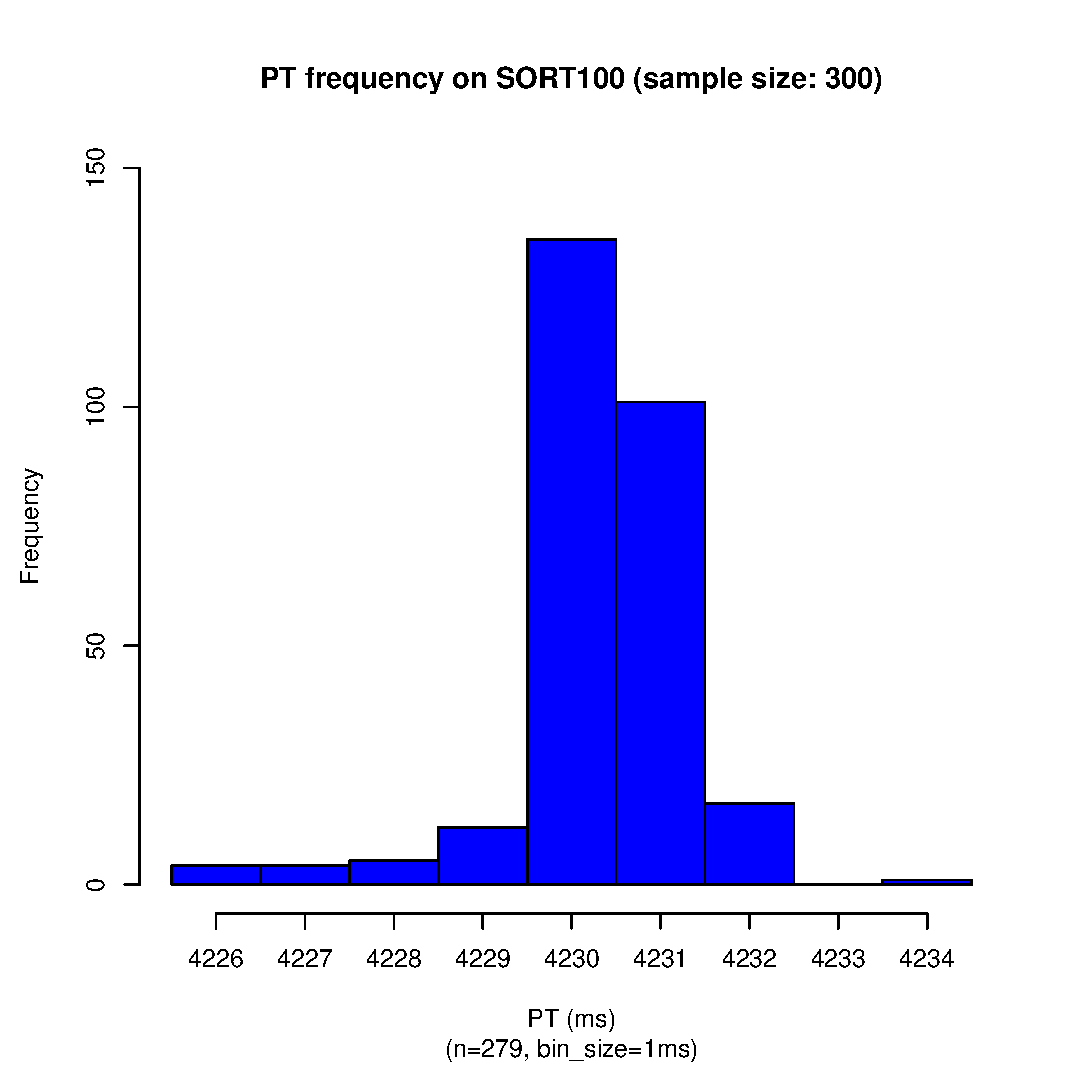
\includegraphics[scale=0.43]{sort100_dist.eps}
%		\label{fig:sort100_dist}
%	}
%	\subfigure[PT frequency on SORT144]{
%		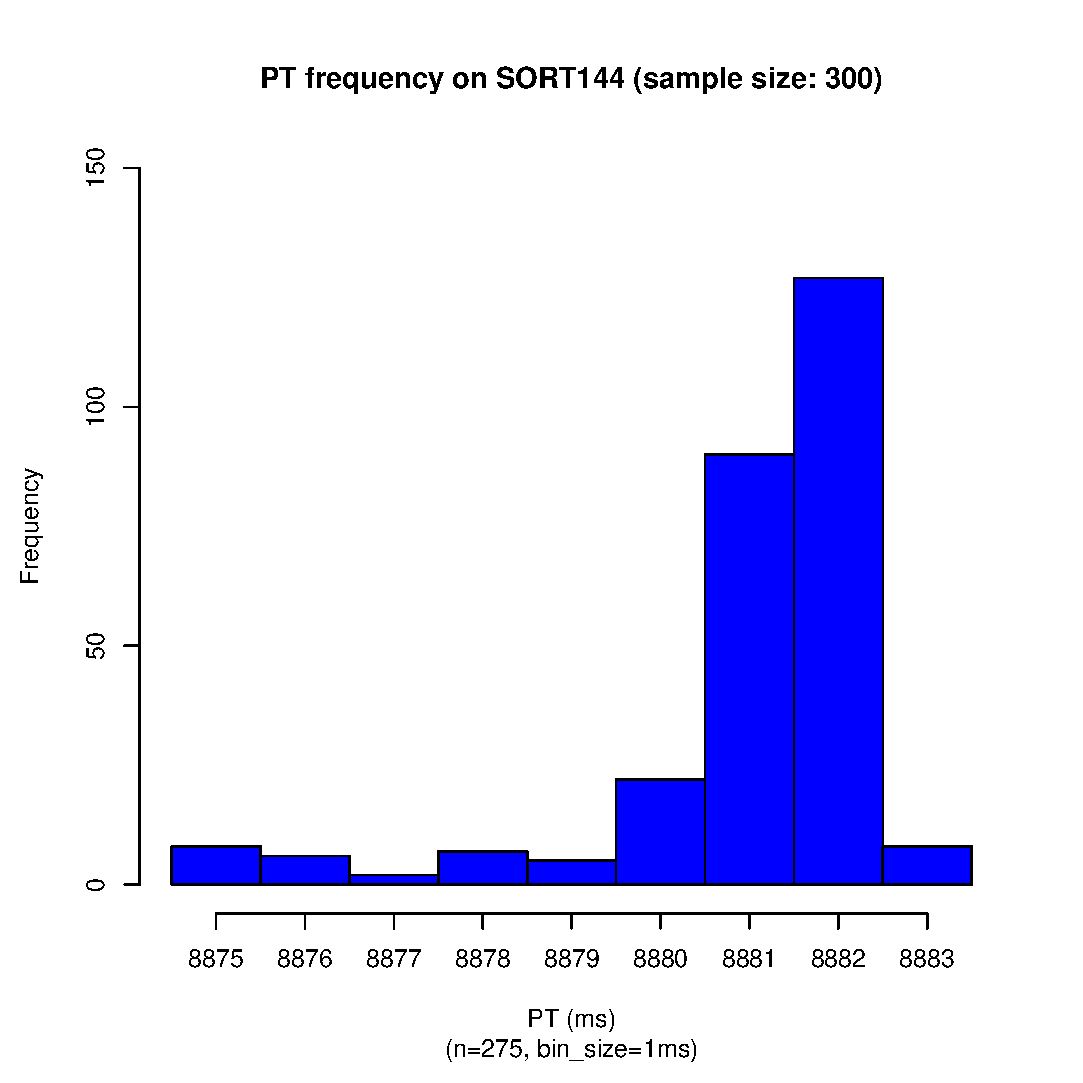
\includegraphics[scale=0.43]{sort144_dist.eps}
%		\label{fig:sort144_dist}
%	}
%	\subfigure[PT frequency on SORT200]{
%		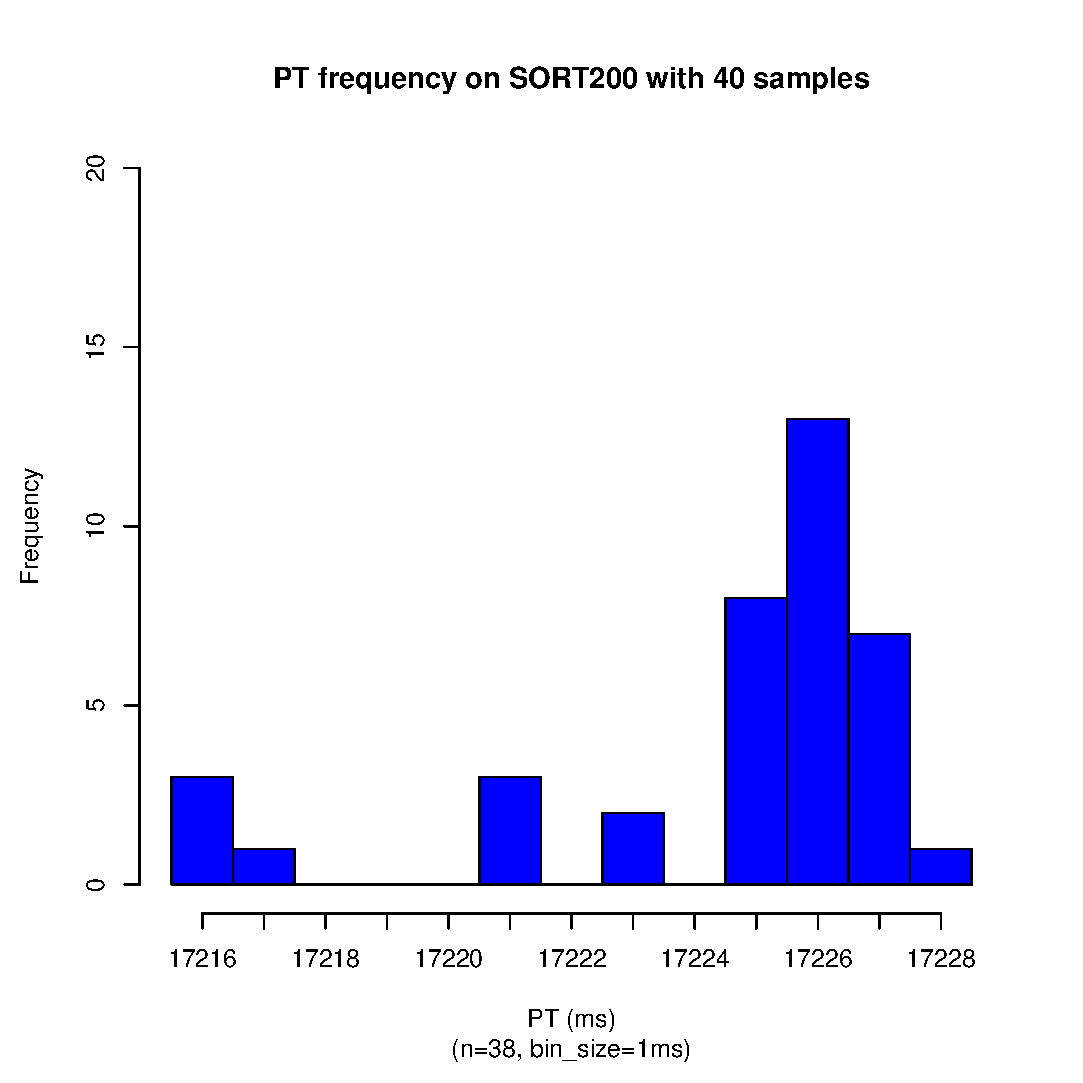
\includegraphics[scale=0.43]{sort200_dist.eps}
%		\label{fig:sort200_dist}
%	}
%	\subfigure[PT frequency on SORT288]{
%		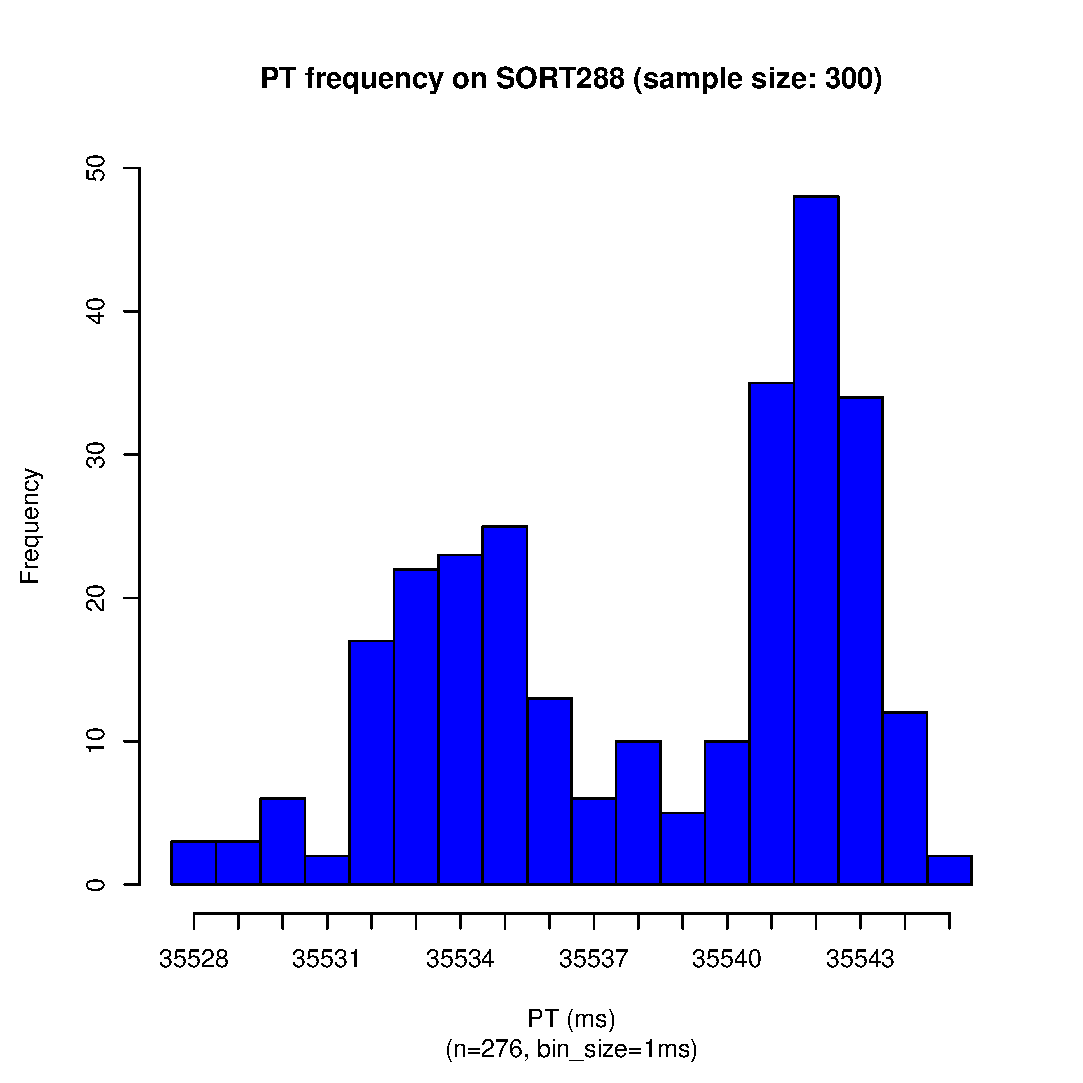
\includegraphics[scale=0.43]{sort288_dist.eps}
%		\label{fig:sort288_dist}
%	}
%	\caption{PT Histograms of SORT25 ... SORT288~\label{fig:sort1}}
%\end{figure}
%
%\clearpage
%\pagebreak
%
%\begin{figure}[h]
%	\centering
%	\subfigure[PT frequency on SORT400]{
%		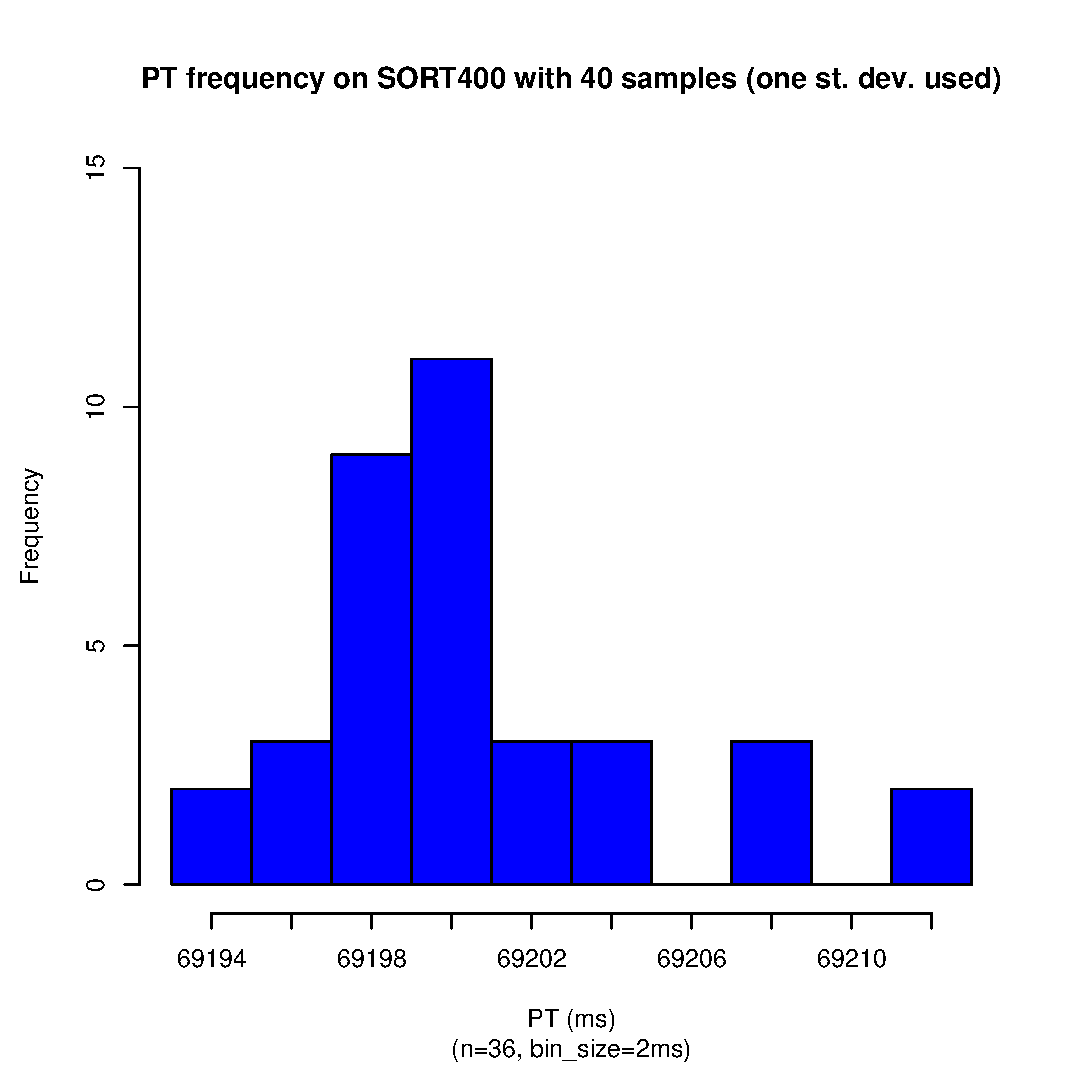
\includegraphics[scale=0.43]{sort400_dist.eps}
%		\label{fig:sort400_dist}
%	}
%	\subfigure[PT frequency on SORT580]{
%		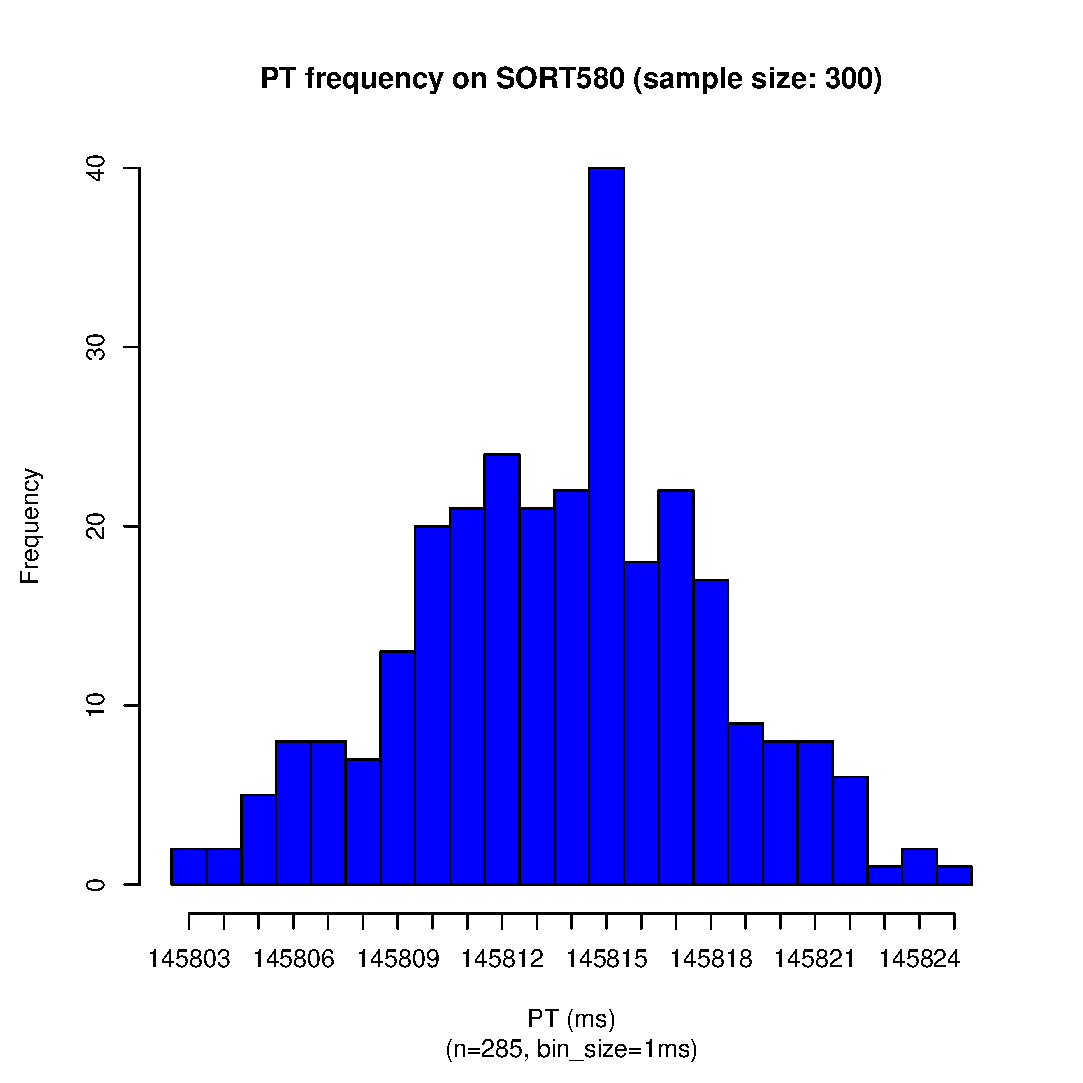
\includegraphics[scale=0.43]{sort580_dist.eps}
%		\label{fig:sort588_dist}
%	}
%	\subfigure[PT frequency on SORT800]{
%		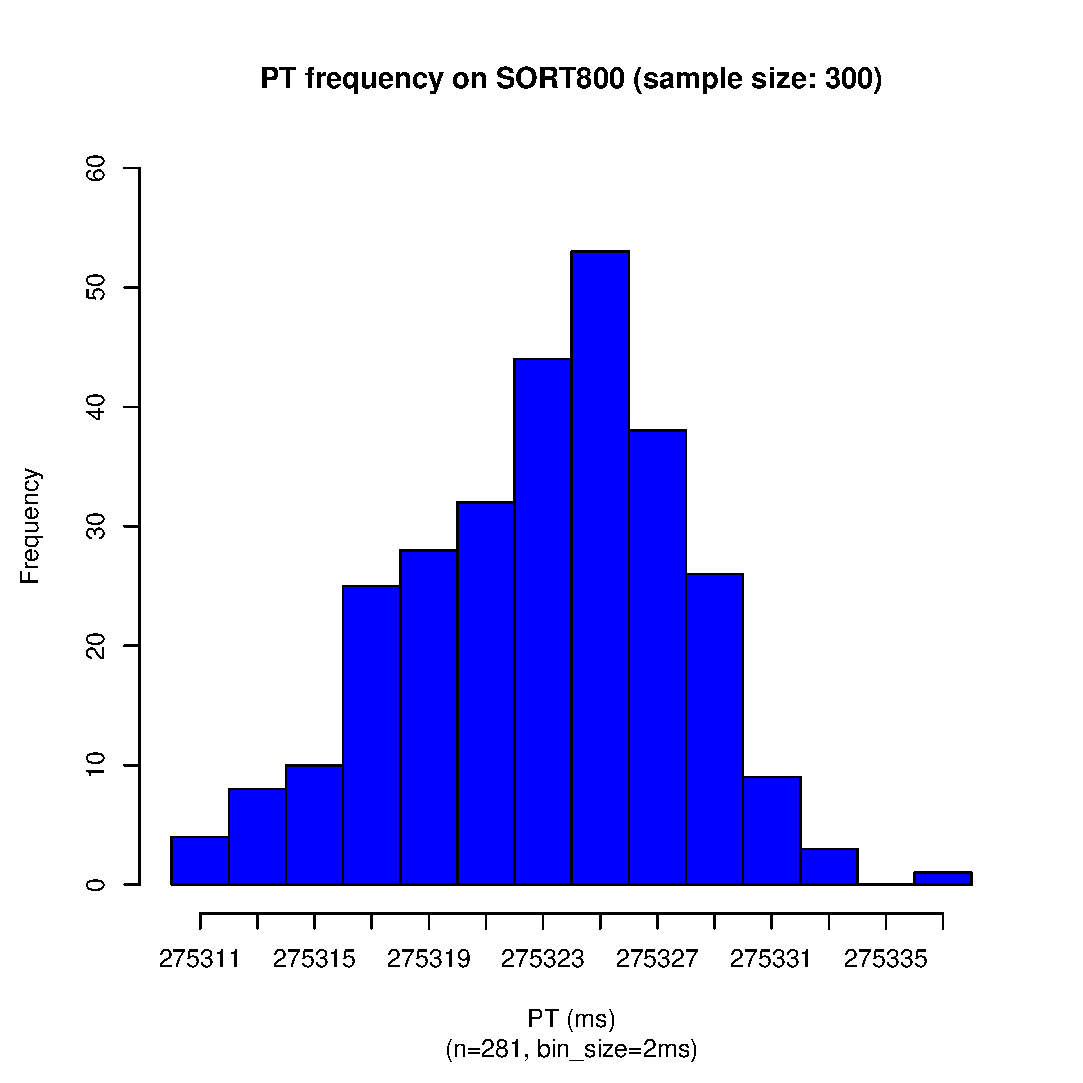
\includegraphics[scale=0.43]{sort800_dist.eps}
%		\label{fig:sort800_dist}
%	}
%	\subfigure[PT frequency on SORT1000]{
%		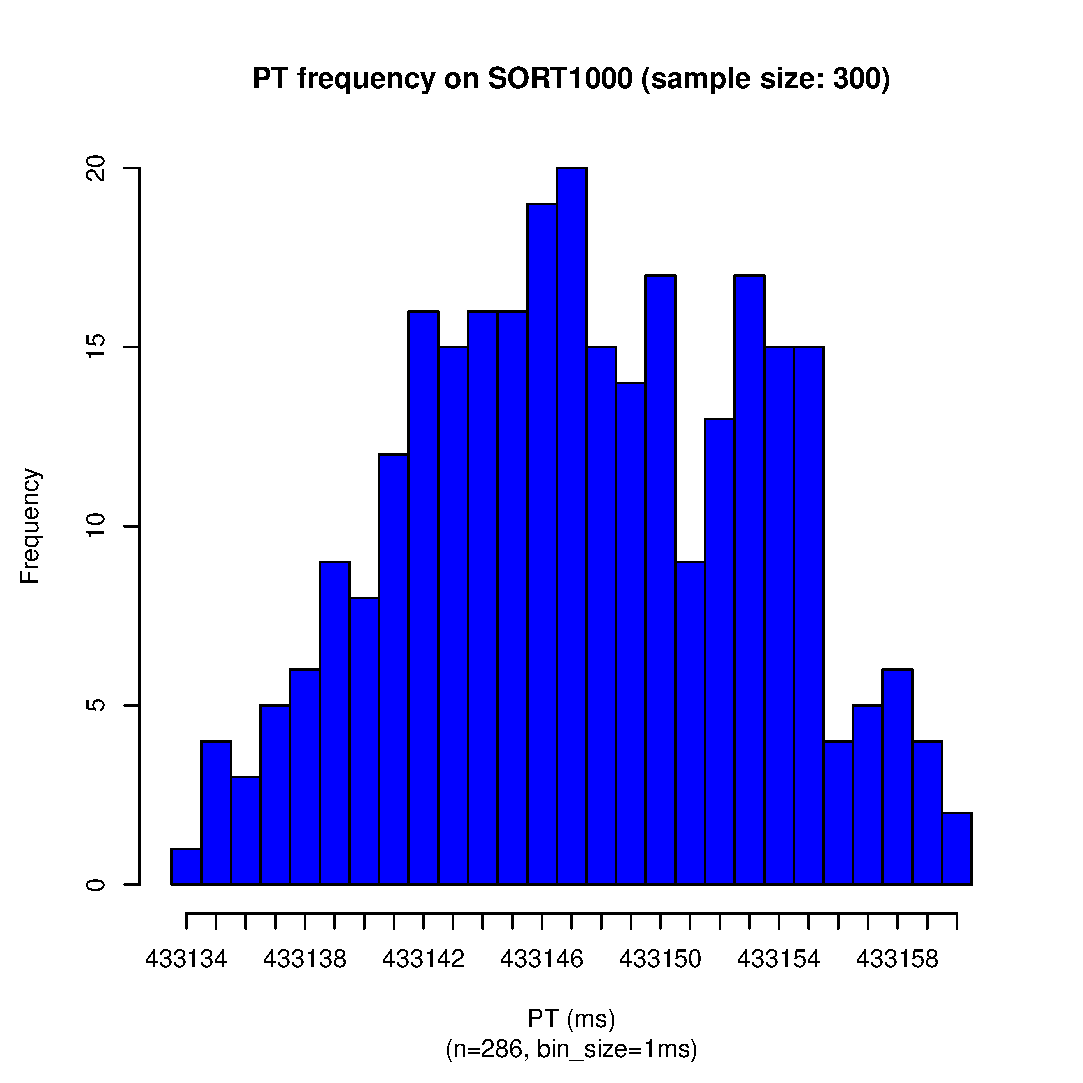
\includegraphics[scale=0.43]{sort1000_dist.eps}
%		\label{fig:sort1000_dist}
%	}
%	\caption{PT Histograms of SORT400 ... SORT1000~\label{fig:sort2}}
%\end{figure}
%
%\begin{figure}[h]
%	\centering
%	\subfigure[PT frequency on SORT1160]{
%		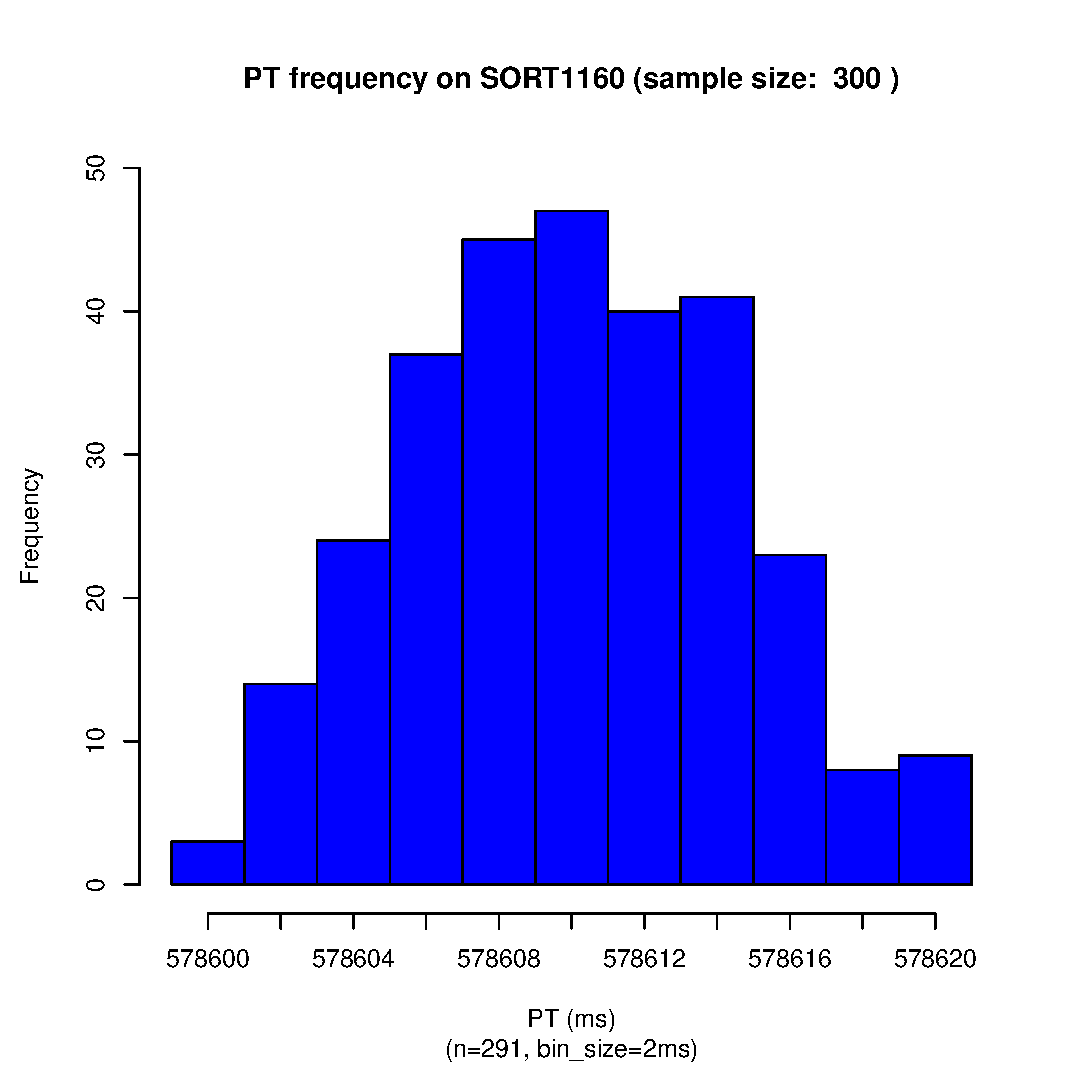
\includegraphics[scale=0.43]{sort1160_dist.eps}
%		\label{fig:sort1160_dist}
%	}
%	\subfigure[PT frequency on SORT2320 (not complete)]{
%		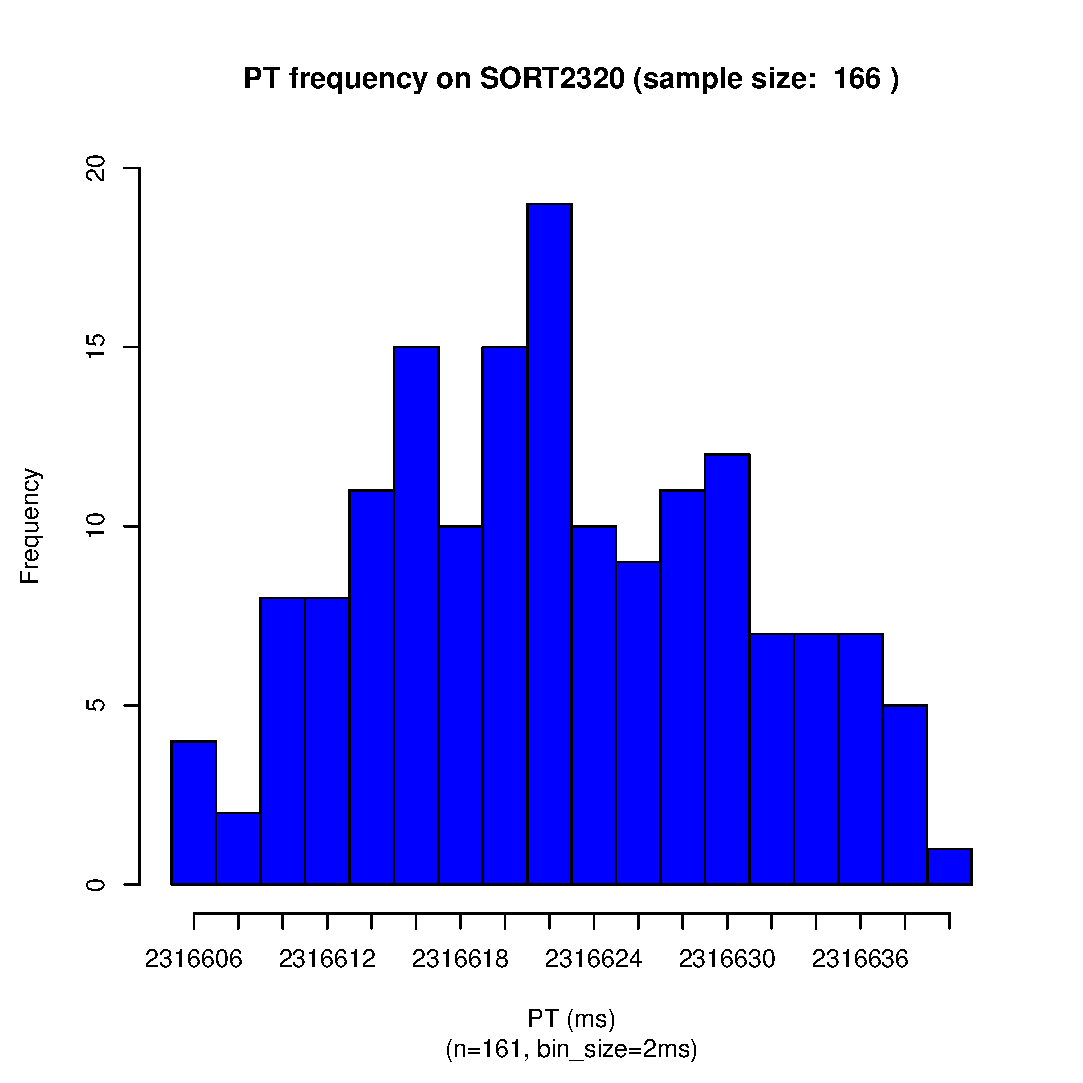
\includegraphics[scale=0.43]{sort2320_dist.eps}
%		\label{fig:sort2320_dist}
%	}
%	\caption{PT Histograms of SORT1160 ... SORT2320~\label{fig:sort3}}
%\end{figure}

%\begin{comment}

%\clearpage
%\pagebreak
%
%\begin{figure}[h]
%	\centering
%	\subfigure[PT frequency on SORT2320 (Will be updated with the rest.)]{
%		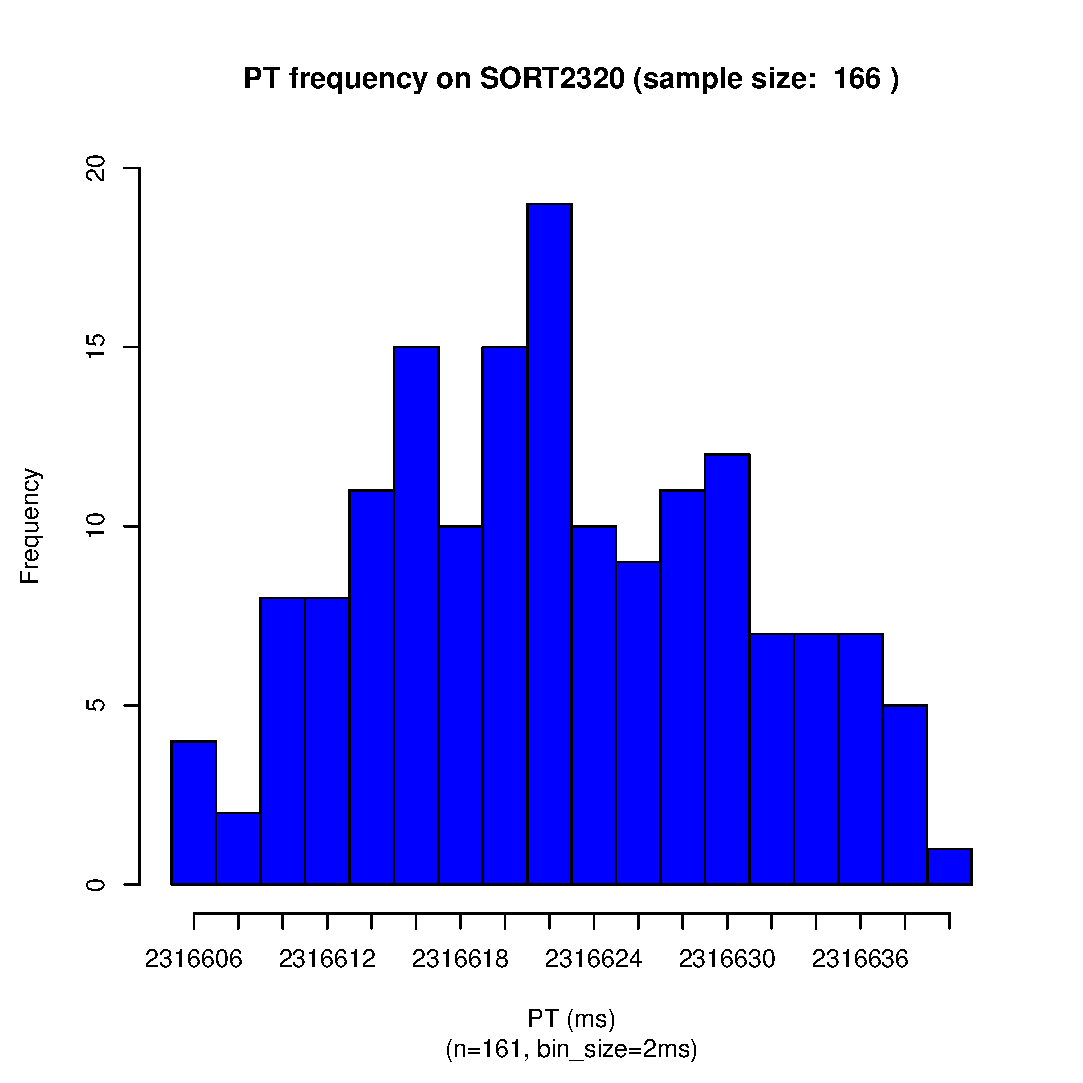
\includegraphics[scale=0.43]{sort2320_dist.eps}
%		\label{fig:sort2320_dist}
%	}
%	\subfigure[PT frequency on SORT3200]{
%		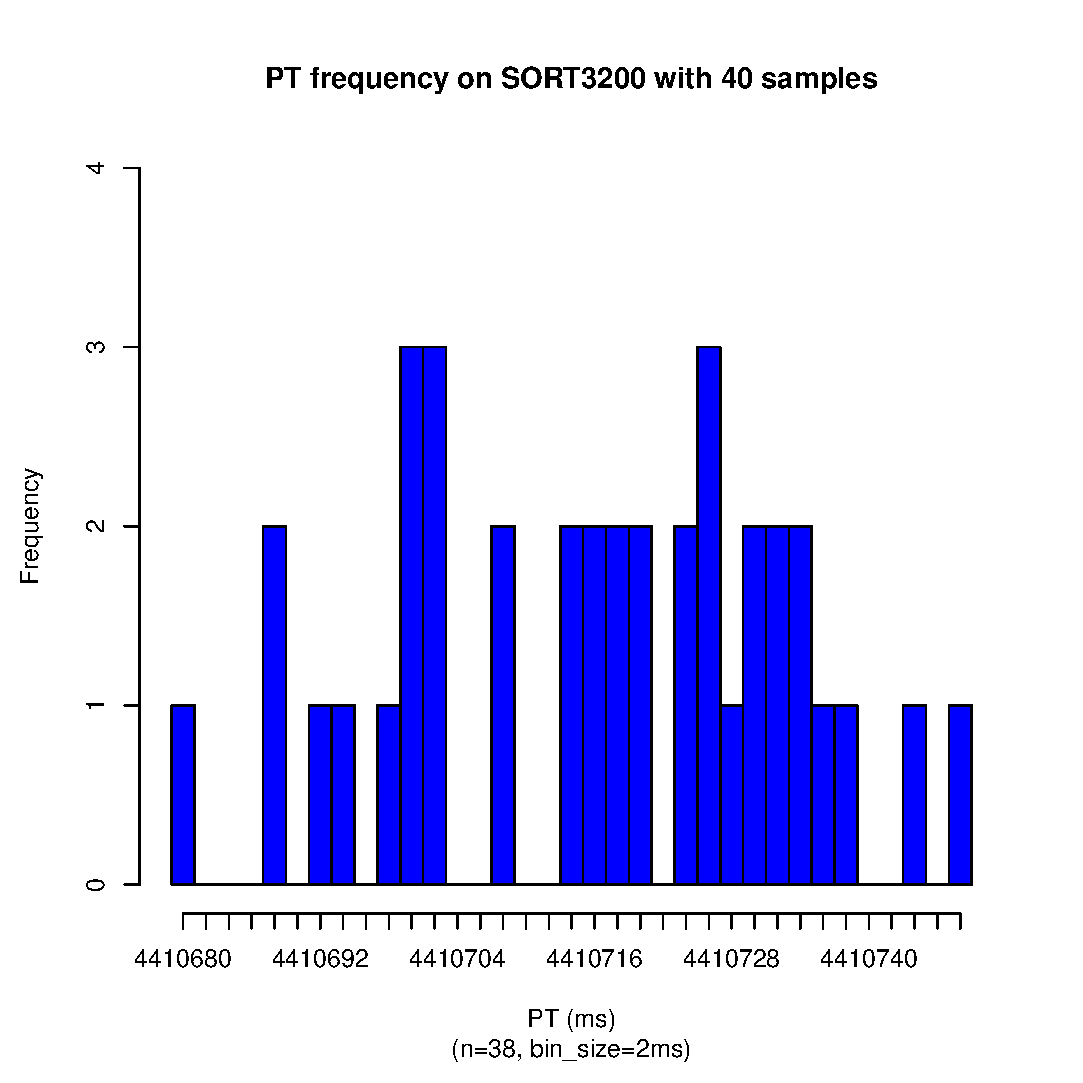
\includegraphics[scale=0.43]{sort3200_dist.eps}
%		\label{fig:sort3200_dist}
%	}
%	\\
%	\subfigure[PT frequency on SORT4640]{
%		%
\includegraphics[scale=0.43]{sort4640_dist.eps}
%		\framebox(200,200){Will be available soon.}
%		\label{fig:sort4640_dist}
%	}
%	\subfigure[PT frequency on SORT6400]{
%		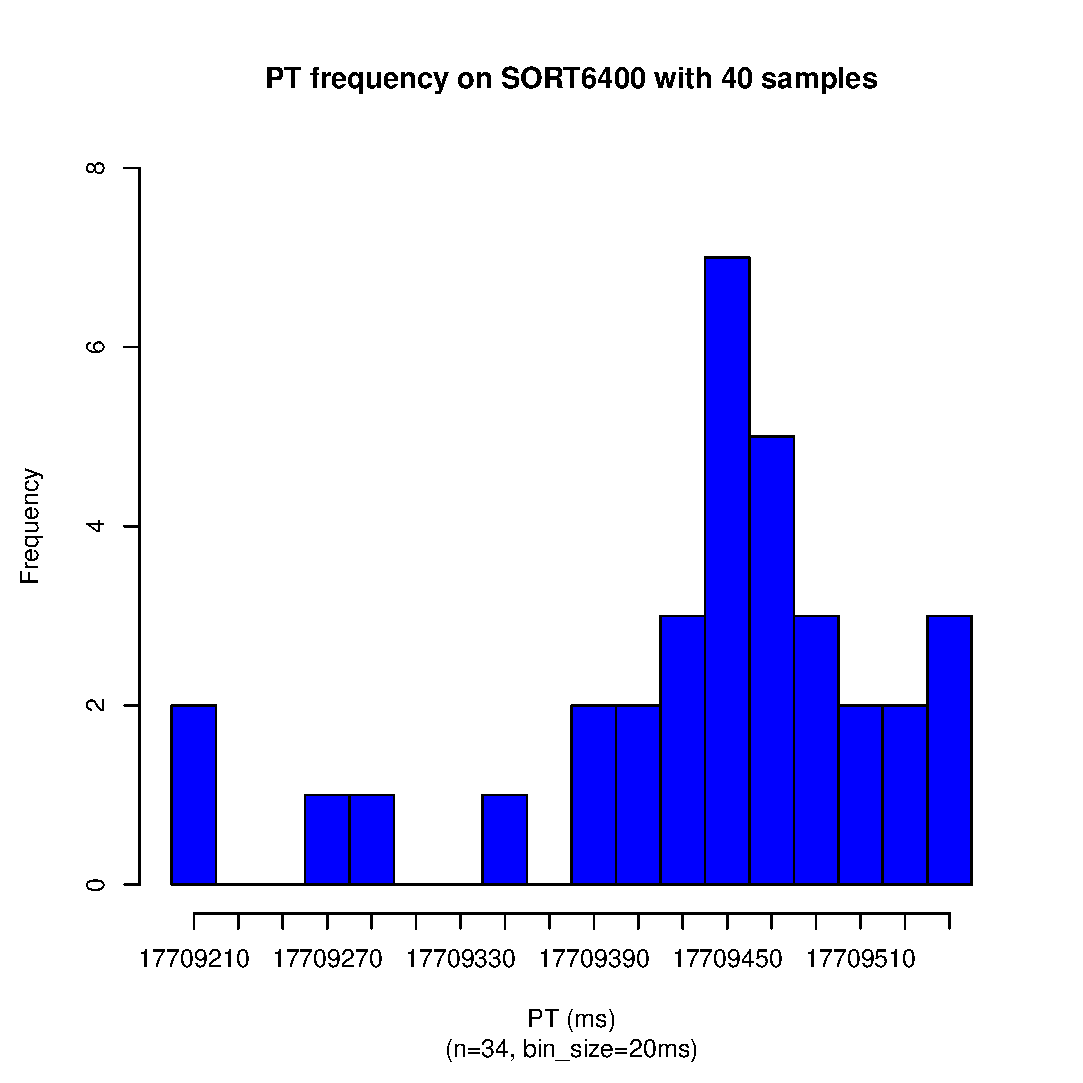
\includegraphics[scale=0.43]{sort6400_dist.eps}
%		\label{fig:sort6400_dist}
%	}
%	\caption{PT Histograms of SORT2320 ... SORT6400~\label{fig:sort3}}
%\end{figure}

\clearpage
\pagebreak

\subsection{Matrix Multiplication~\label{sec:mm}} 

This section shows a series of histograms of 
the execution times of an matrix multiplication program. 
We used the same sample size for each input size of this program: i.e., 40 iterations. 
For simplicity, we used two square matrices for performing their multiplication in the program.  
We also varied the input sizes of each of the two matrices: 
from 1K$\times$1K to 8K$\times$8K integer elements that are also randomly generated. 
Note that each matrix multiplication program for a specific size is called MAT{\it xyyyy}, 
where {\it x} indicates which major, specifically {\em column} vs. {\em row}, is used, and {\it yyyy}, how large a given matrix is. 
For instance, MATC1000 represents a matrix multiplication program 
in column major over two square matrices having 1,000 integer (random) 
elements in a row (and a column). 

\pagebreak

\subsubsection{Column Major}

Figure~\ref{fig:matc} shows a series of 
histograms of the execution times measured on 
the same matrix multiplication program in column major 
as the input sizes grows. 

%\begin{figure}[h]
%	\centering
%	\subfigure[PT frequency on MATC250]{
%		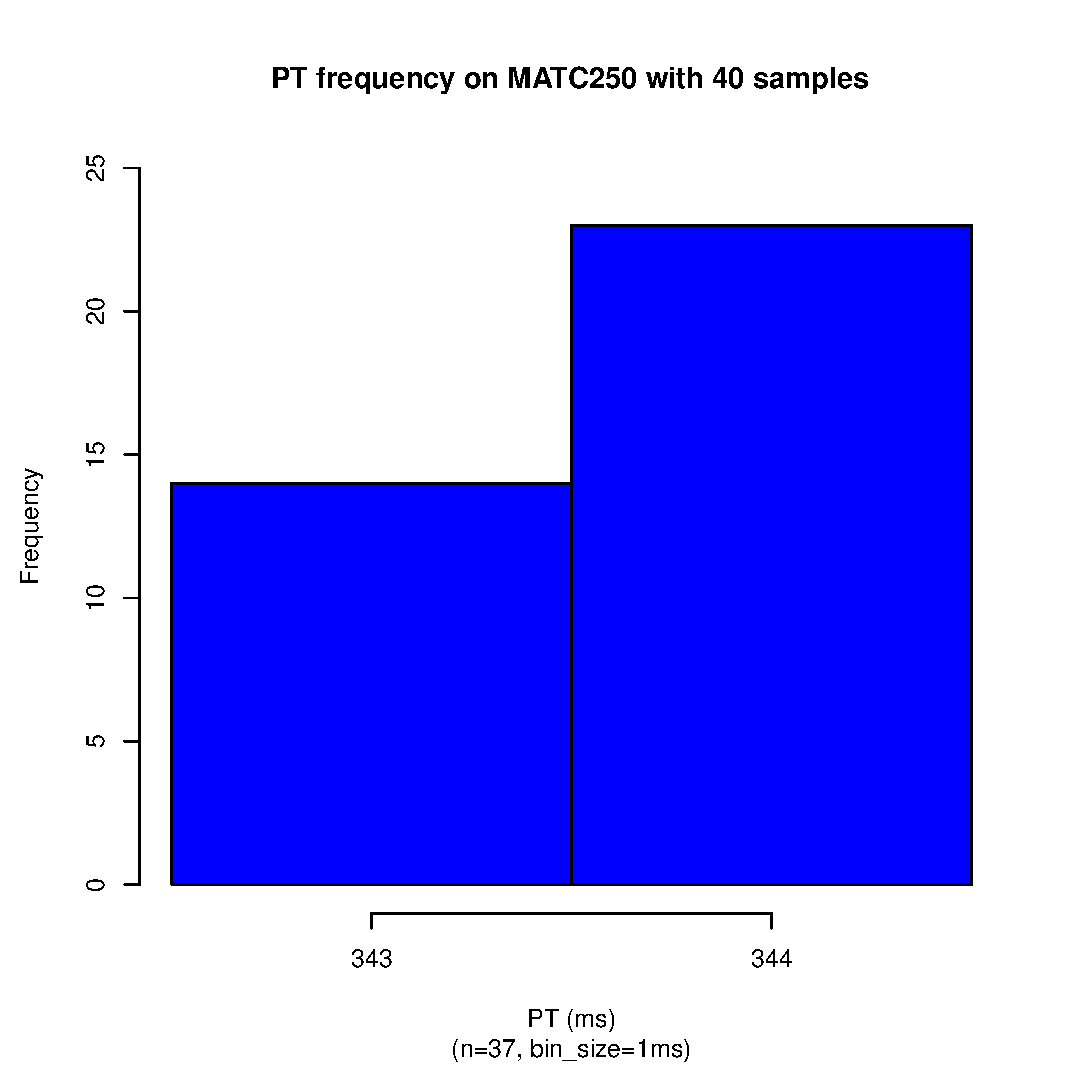
\includegraphics[scale=0.43]{matc250_dist.eps}
%		\label{fig:matc250_dist}
%	}
%	\subfigure[PT frequency on MATC500]{
%		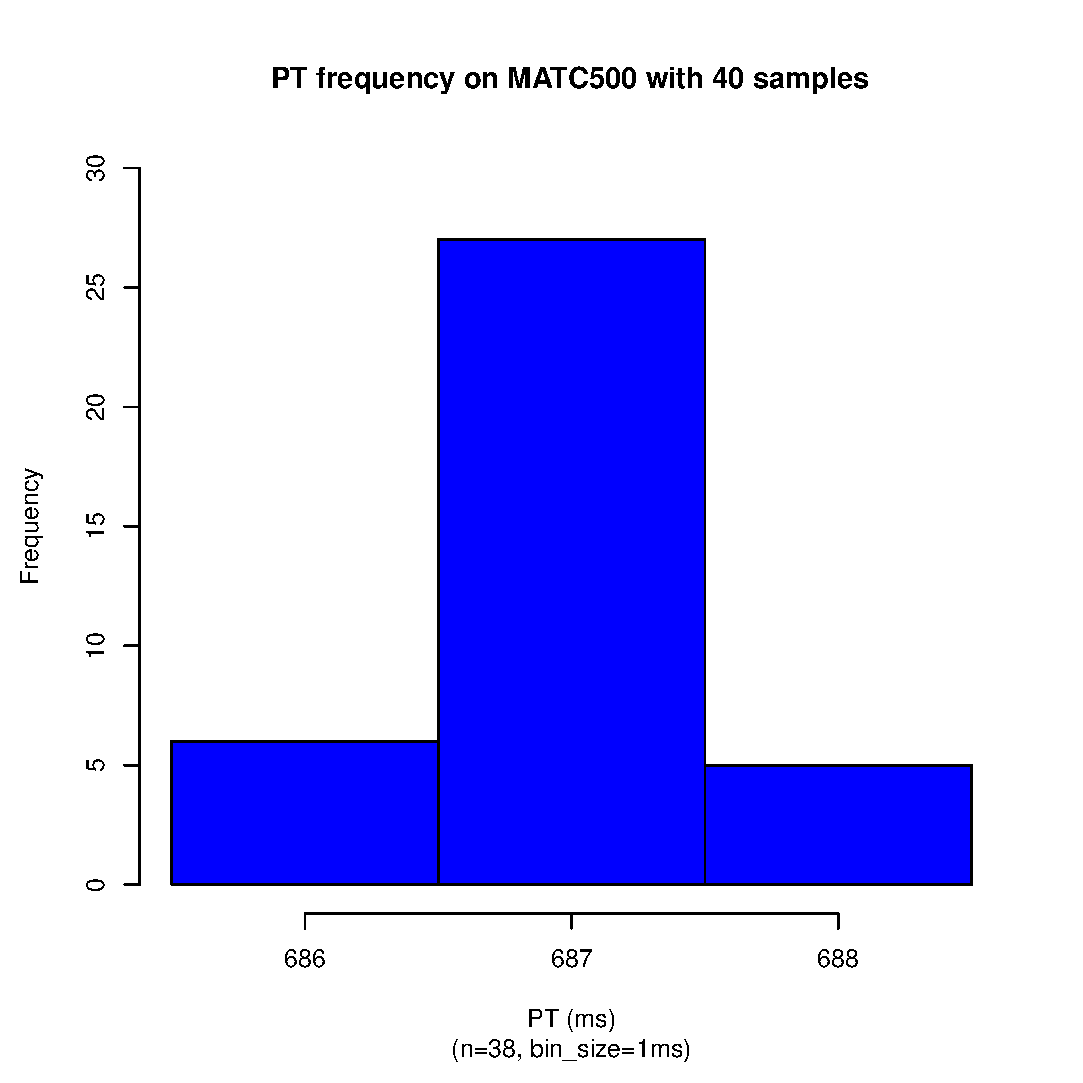
\includegraphics[scale=0.43]{matc500_dist.eps}
%		\label{fig:matc500_dist}
%	}
%	\subfigure[PT frequency on MATC1024]{
%		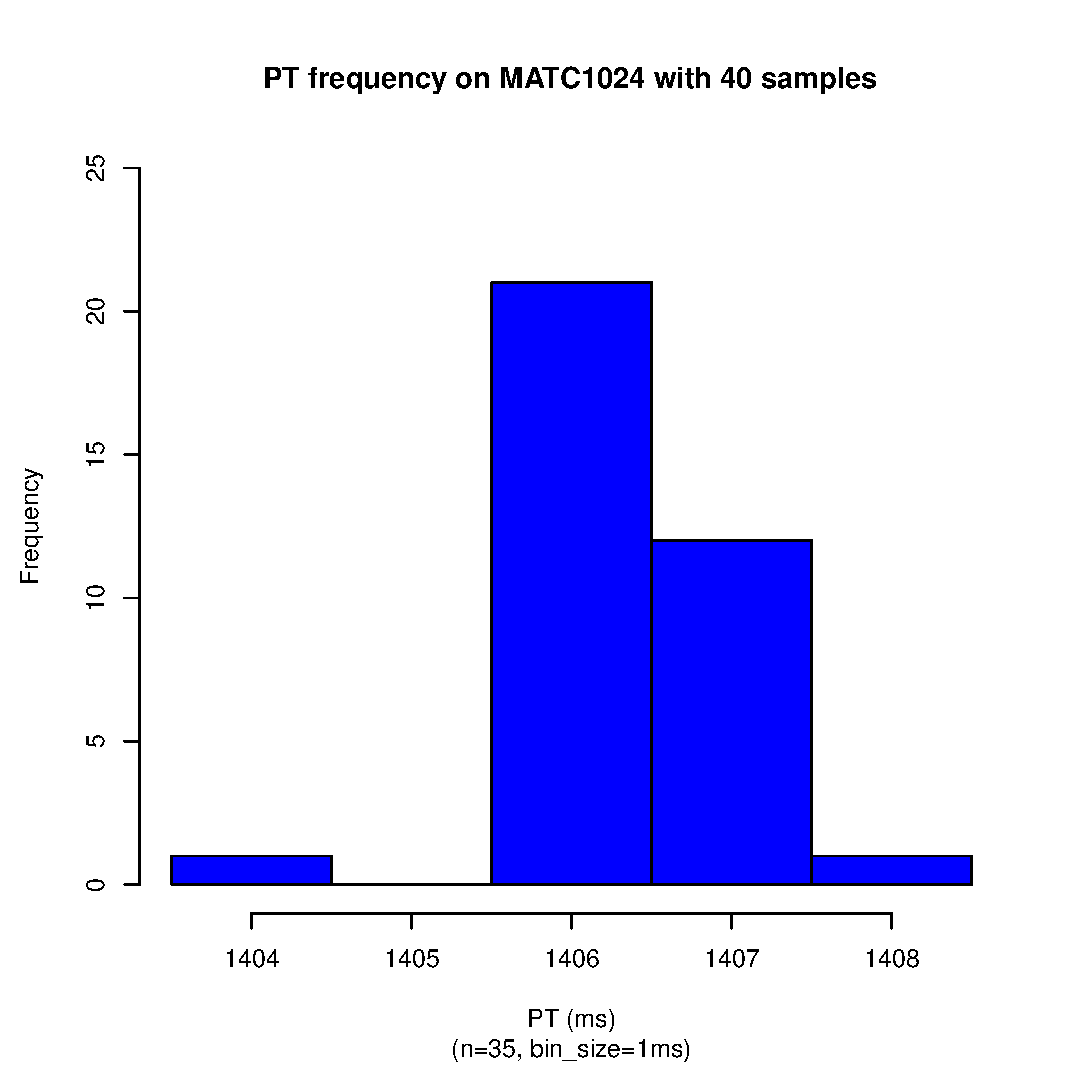
\includegraphics[scale=0.43]{matc1024_dist2.eps}
%		\label{fig:matc1024_dist}
%	}
%	\subfigure[PT frequency on MATC1440]{
%		\includegraphics[scale=0.43]{matc1440_dist.eps}
%		\label{fig:matc1440_dist}
%	}
%	\caption{PT Histograms of MATC250 ... MATC1440~\label{fig:matc}}
%\end{figure}
%
%\begin{figure}[h]
%	\centering
%	\subfigure[PT frequency on MATC2048]{
%		\includegraphics[scale=0.43]{matc2048_dist2.eps}
%		\label{fig:matc2048_dist}
%	}
%	\subfigure[PT frequency on MATC2880]{
%		\includegraphics[scale=0.43]{matc2880_dist.eps}
%		\label{fig:matc2880_dist}
%	}	
%	\subfigure[PT frequency on MATC4096]{
%		\includegraphics[scale=0.43]{matc4096_dist2.eps}
%		\label{fig:matc4096_dist}
%	}	
%	\subfigure[PT frequency on MATC5760]{
%		\includegraphics[scale=0.43]{matc5760_dist.eps}
%		\label{fig:matc5760_dist}
%	}	
%	\caption{PT Histograms of MATC2048 ... MATC5760~\label{fig:matc2}}
%\end{figure}
%
%\begin{figure}[h]
%	\centering
%	\subfigure[PT frequency on MATC8192]{
%		\includegraphics[scale=0.43]{matc8192_dist2.eps}
%		\label{fig:matc8192_dist}
%	}
%	\subfigure[PT frequency on MATC11520]{
%		\includegraphics[scale=0.43]{matc11520_dist.eps}
%		\label{fig:matc11520_dist}
%	}
%	\subfigure[PT frequency on MATC16000]{
%		\includegraphics[scale=0.43]{matc16000_dist.eps}
%		\label{fig:matc16000_dist}
%	}
%	\subfigure[PT frequency on MATC23040]{
%		\includegraphics[scale=0.43]{matc23040_dist.eps}
%		\label{fig:matc23040_dist}
%	}
%	\caption{PT Histograms of MATC8192 ... MATC23040~\label{fig:matc3}}
%\end{figure}

\begin{figure}[h]
	\centering
	\subfigure[PT frequency on MATC1K]{
		\includegraphics[scale=0.43]{matc1024_dist.eps}
		\label{fig:matc1k_dist}
	}
	\subfigure[PT frequency on MATC2K]{
		\includegraphics[scale=0.43]{matc2048_dist.eps}
		\label{fig:matc2k_dist}
	}
	\subfigure[PT frequency on MATC4K]{
		\includegraphics[scale=0.43]{matc4096_dist.eps}
		\label{fig:matc4k_dist}
	}
	\subfigure[PT frequency on MATC8K]{
		\includegraphics[scale=0.43]{matc8192_dist.eps}
		\label{fig:matc8k_dist}
	}
	\caption{PT Histograms of MATC1024 ... MATC8192~\label{fig:matc}}
\end{figure}

\clearpage
\pagebreak

\subsubsection{Row Major}

Figure~\ref{fig:matc} shows a series of 
histograms of the execution times measured on 
the same matrix multiplication program in row major as the input sizes grows. 

%\begin{figure}[h]
%	\centering
%	\subfigure[PT frequency on MATR250]{
%		\includegraphics[scale=0.43]{matr250_dist.eps}
%		\label{fig:matr250_dist}
%	}
%	\subfigure[PT frequency on MATR500]{
%		\includegraphics[scale=0.43]{matr500_dist.eps}
%		\label{fig:matr500_dist}
%	}
%	\subfigure[PT frequency on MATR1024]{
%		\includegraphics[scale=0.43]{matr1024_dist2.eps}
%		\label{fig:matr1024_dist}
%	}
%	\subfigure[PT frequency on MATR1440]{
%		\includegraphics[scale=0.43]{matr1440_dist.eps}
%		\label{fig:matr1440_dist}
%	}
%	\caption{PT Histograms of MATR250 ... MATR1440~\label{fig:matr}}
%\end{figure}

%\begin{figure}[h]
%	\centering
%	\subfigure[PT frequency on MATR2048]{
%		\includegraphics[scale=0.43]{matr2048_dist2.eps}
%		\label{fig:matr2048_dist}
%	}
%	\subfigure[PT frequency on MATR2880]{
%		\includegraphics[scale=0.43]{matr2880_dist.eps}
%		\label{fig:matr2880_dist}
%	}	
%	\subfigure[PT frequency on MATR4096]{
%		\includegraphics[scale=0.43]{matr4096_dist2.eps}
%		\label{fig:matr4096_dist}
%	}	
%	\subfigure[PT frequency on MATR5760]{
%		\includegraphics[scale=0.43]{matr5760_dist.eps}
%		\label{fig:matr5760_dist}
%	}	
%	\caption{PT Histograms of MATR2048 ... MATR5760~\label{fig:matr2}}
%\end{figure}
%
%\begin{figure}[h]
%	\centering
%	\subfigure[PT frequency on MATR8192]{
%		\includegraphics[scale=0.43]{matr8192_dist2.eps}
%		\label{fig:matr8192_dist}
%	}
%	\subfigure[PT frequency on MATR11520]{
%		\includegraphics[scale=0.43]{matr11520_dist.eps}
%		\label{fig:matr11520_dist}
%	}	
%	\subfigure[PT frequency on MATR16000]{
%		\includegraphics[scale=0.43]{matr16000_dist.eps}
%		\label{fig:matr16000_dist}
%	}
%	\subfigure[PT frequency on MATR23040]{
%		\includegraphics[scale=0.43]{matr23040_dist.eps}
%		\label{fig:matr23040_dist}
%	}
%	\caption{PT Histograms of MATR8192 ... MATR23040~\label{fig:matr3}}
%\end{figure}

\begin{figure}[h]
	\centering
	\subfigure[PT frequency on MATR1K]{
		\includegraphics[scale=0.43]{matr1024_dist.eps}
		\label{fig:matr1k_dist}
	}
	\subfigure[PT frequency on MATR2K]{
		\includegraphics[scale=0.43]{matr2048_dist.eps}
		\label{fig:matr2k_dist}
	}
	\subfigure[PT frequency on MATR4K]{
		\includegraphics[scale=0.43]{matr4096_dist.eps}
		\label{fig:matr4k_dist}
	}
	\subfigure[PT frequency on MATR8K]{
		\includegraphics[scale=0.43]{matr8192_dist.eps}
		\label{fig:matr8k_dist}
	}
	\caption{PT Histograms of MATR1K ... MATR8K~\label{fig:matr}}
\end{figure}

\clearpage
\pagebreak

%\end{comment}

\bibliographystyle{abbrv}
\newcommand{\etalchar}[1]{$^{#1}$}
\begin{thebibliography}{99}
\vspace{0.1em}
%\bibitem
%{Avnur:2000:ECA:342009.335420}
%{Sedona}
%Young-Kyoon Suh, ``SEDONA: A Novel Protocol for Identifying Infrequent, Long-running Daemons on a Linux System'', in {\em IEICE Transactions on Information Systems}, Vol. 100D, No. 9, pp.~??--??, 2017.
%\vspace{0.1em}
\bibitem
%{Avnur:2000:ECA:342009.335420}
{EMP}
Young-Kyoon Suh, Richard T. Snodgrass, John Kececioglu, Peter J. Downey, Rob S. Maier, and Cheng Yi, ``EMP: Execution Time Measurement Protocol for Compute-Bound Programs'', in {\em Software: Practice and Experience}, 47(4):559--597, 2017.
\bibitem
%{Avnur:2000:ECA:342009.335420}
{Metrology}
Sabah Currim,Richard T. Snodgrass, Young-Kyoon Suh, and Rui Zhang, ``DBMS Metrology: Measuring Query Time'', in {\em ACM Transactions on Database Systems}, 42(1):3:1--42(+8), 2017.
\end{thebibliography}

\end{document}